\chapter{Results \& Discussions}

\begin{comment}
\indent\indent From Chapter 2 onwards, every chapter should start with an introduction paragraph. This paragraph should brief about the flow of the chapter. This introduction can be limited within 4 to 5 sentences. The chapter heading should be appropriately modified (a sample heading is shown for this chapter).But don't start the introduction paragraph in the chapters 2 to end with "This chapter deals with....". Instead you should bring in the highlights of the chapter in the introduction paragraph.
\end{comment}
Analyzing both architectural and accelerator-level outcomes is essential to validate the design choices and methodologies established in earlier stages. This chapter presents detailed results from the FPGA architecture exploration using the VTR toolchain, comparing delay, area, and frequency metrics across three different architectures and multiple ML-representative benchmarks. It also includes a comprehensive evaluation of the Manojavam accelerator, reporting its FPGA and ASIC performance in terms of throughput, power, resource utilization, and execution time. Comparative studies with CPU and GPU platforms further highlight the accelerator's effectiveness in real-world PCA workloads.


%% START CONTENT HERE
\section{Results from FPGA Architectural Exploration}
This section presents the performance analysis of benchmark circuits mapped to three target FPGA architectures — Intel Stratix-10, 4-bit Single Carry Chain, and 4-bit Double Carry Chain — using the VTR toolchain. The benchmarks span arithmetic workloads including adder trees and FIR filters (with both built-in and Wallace tree multipliers). Evaluation is based on three key metrics: critical path delay, area (in MWTA), and maximum operational frequency. The results offer insights into the relationship between architecture design and workload characteristics.

\subsection{Critical Path Delays in Adder Trees}
As seen in Fig.\ref{fig:critical-path-delays-of-2-level-adder-trees-across-bitwidhts}, which plots the critical path delay of 2-level adder trees across increasing bit-widths, the Stratix-10 architecture generally exhibits higher delay compared to the custom 4-bit carry chain architectures. The 4-bit Single Carry Chain shows consistently lower delay up to medium operand sizes, while the 4-bit Double Carry Chain begins to outperform it as operand width increases. This suggests that the parallelism enabled by the double carry structure becomes more effective at reducing depth-dependent delay in larger adders.

\begin{figure}
	\centerline{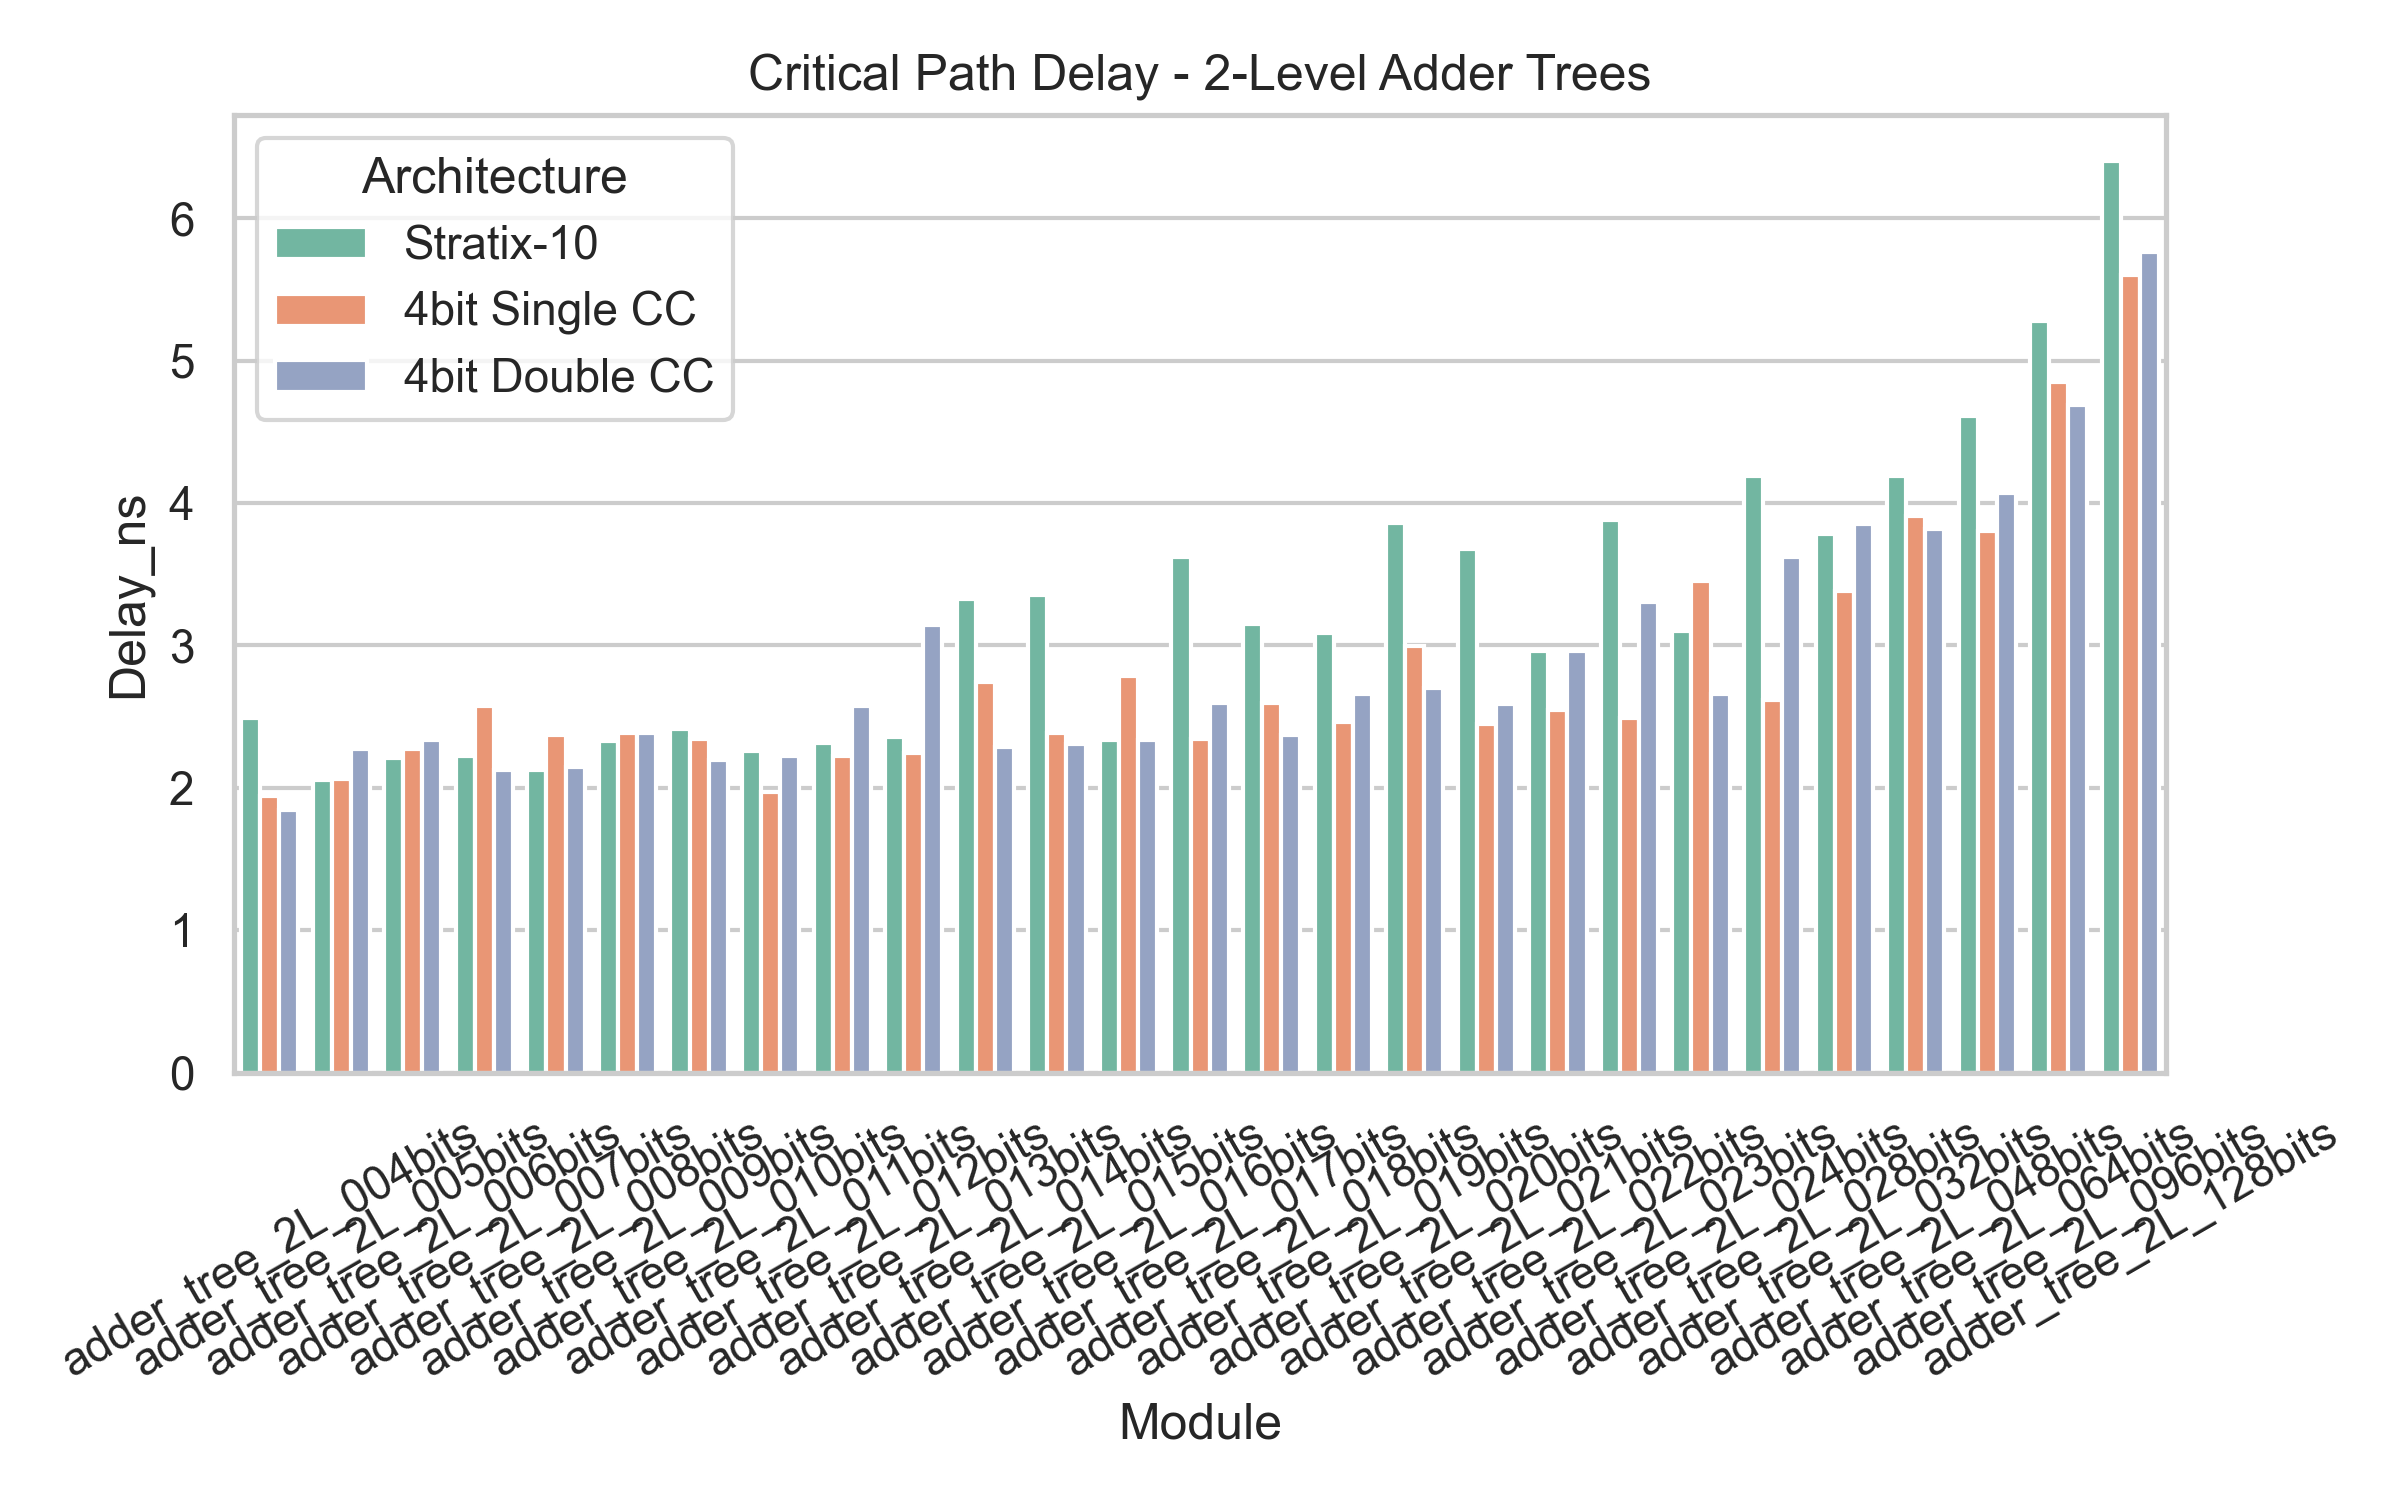
\includegraphics[scale = 0.75]{Figures/adder_trees_2lvl_delay_bar_plt.png}}
	\caption{Critical Path Delays of 2-Level Adder Trees across Bitwidths}
	\label{fig:critical-path-delays-of-2-level-adder-trees-across-bitwidhts}
\end{figure}

For small operand sizes (e.g., 4 to 16 bits), all three architectures show comparable performance, indicating minimal carry chain depth. However, as the operand width grows beyond 64 bits, the benefit of specialized arithmetic routing becomes more apparent, particularly in the Double Carry Chain, which maintains a shallower critical path thanks to its dual-path propagation. This validates the architectural benefit of embedding multiple carry chains in performance-critical datapaths.

\subsection{Area in Adder Trees}
Fig.\ref{fig:Area-(MWTA)-Consumption-of-3-Level-Adder-Trees-across-Architectures} illustrates the area consumption of 3-level adder trees across the three architectures. All architectures show an expected exponential increase in area as operand bit-width increases. However, the difference in area between architectures remains relatively modest for small to mid-sized adders. Notably, the 4-bit Double Carry Chain tends to consume slightly more area than the Single Carry variant, a trade-off resulting from its more complex internal logic structure and wider data paths. Stratix-10, despite being a highly capable general-purpose FPGA, does not show superior area efficiency in this context, suggesting its resources are optimized for broader flexibility rather than arithmetic compactness.

\begin{figure}[H]
	\centerline{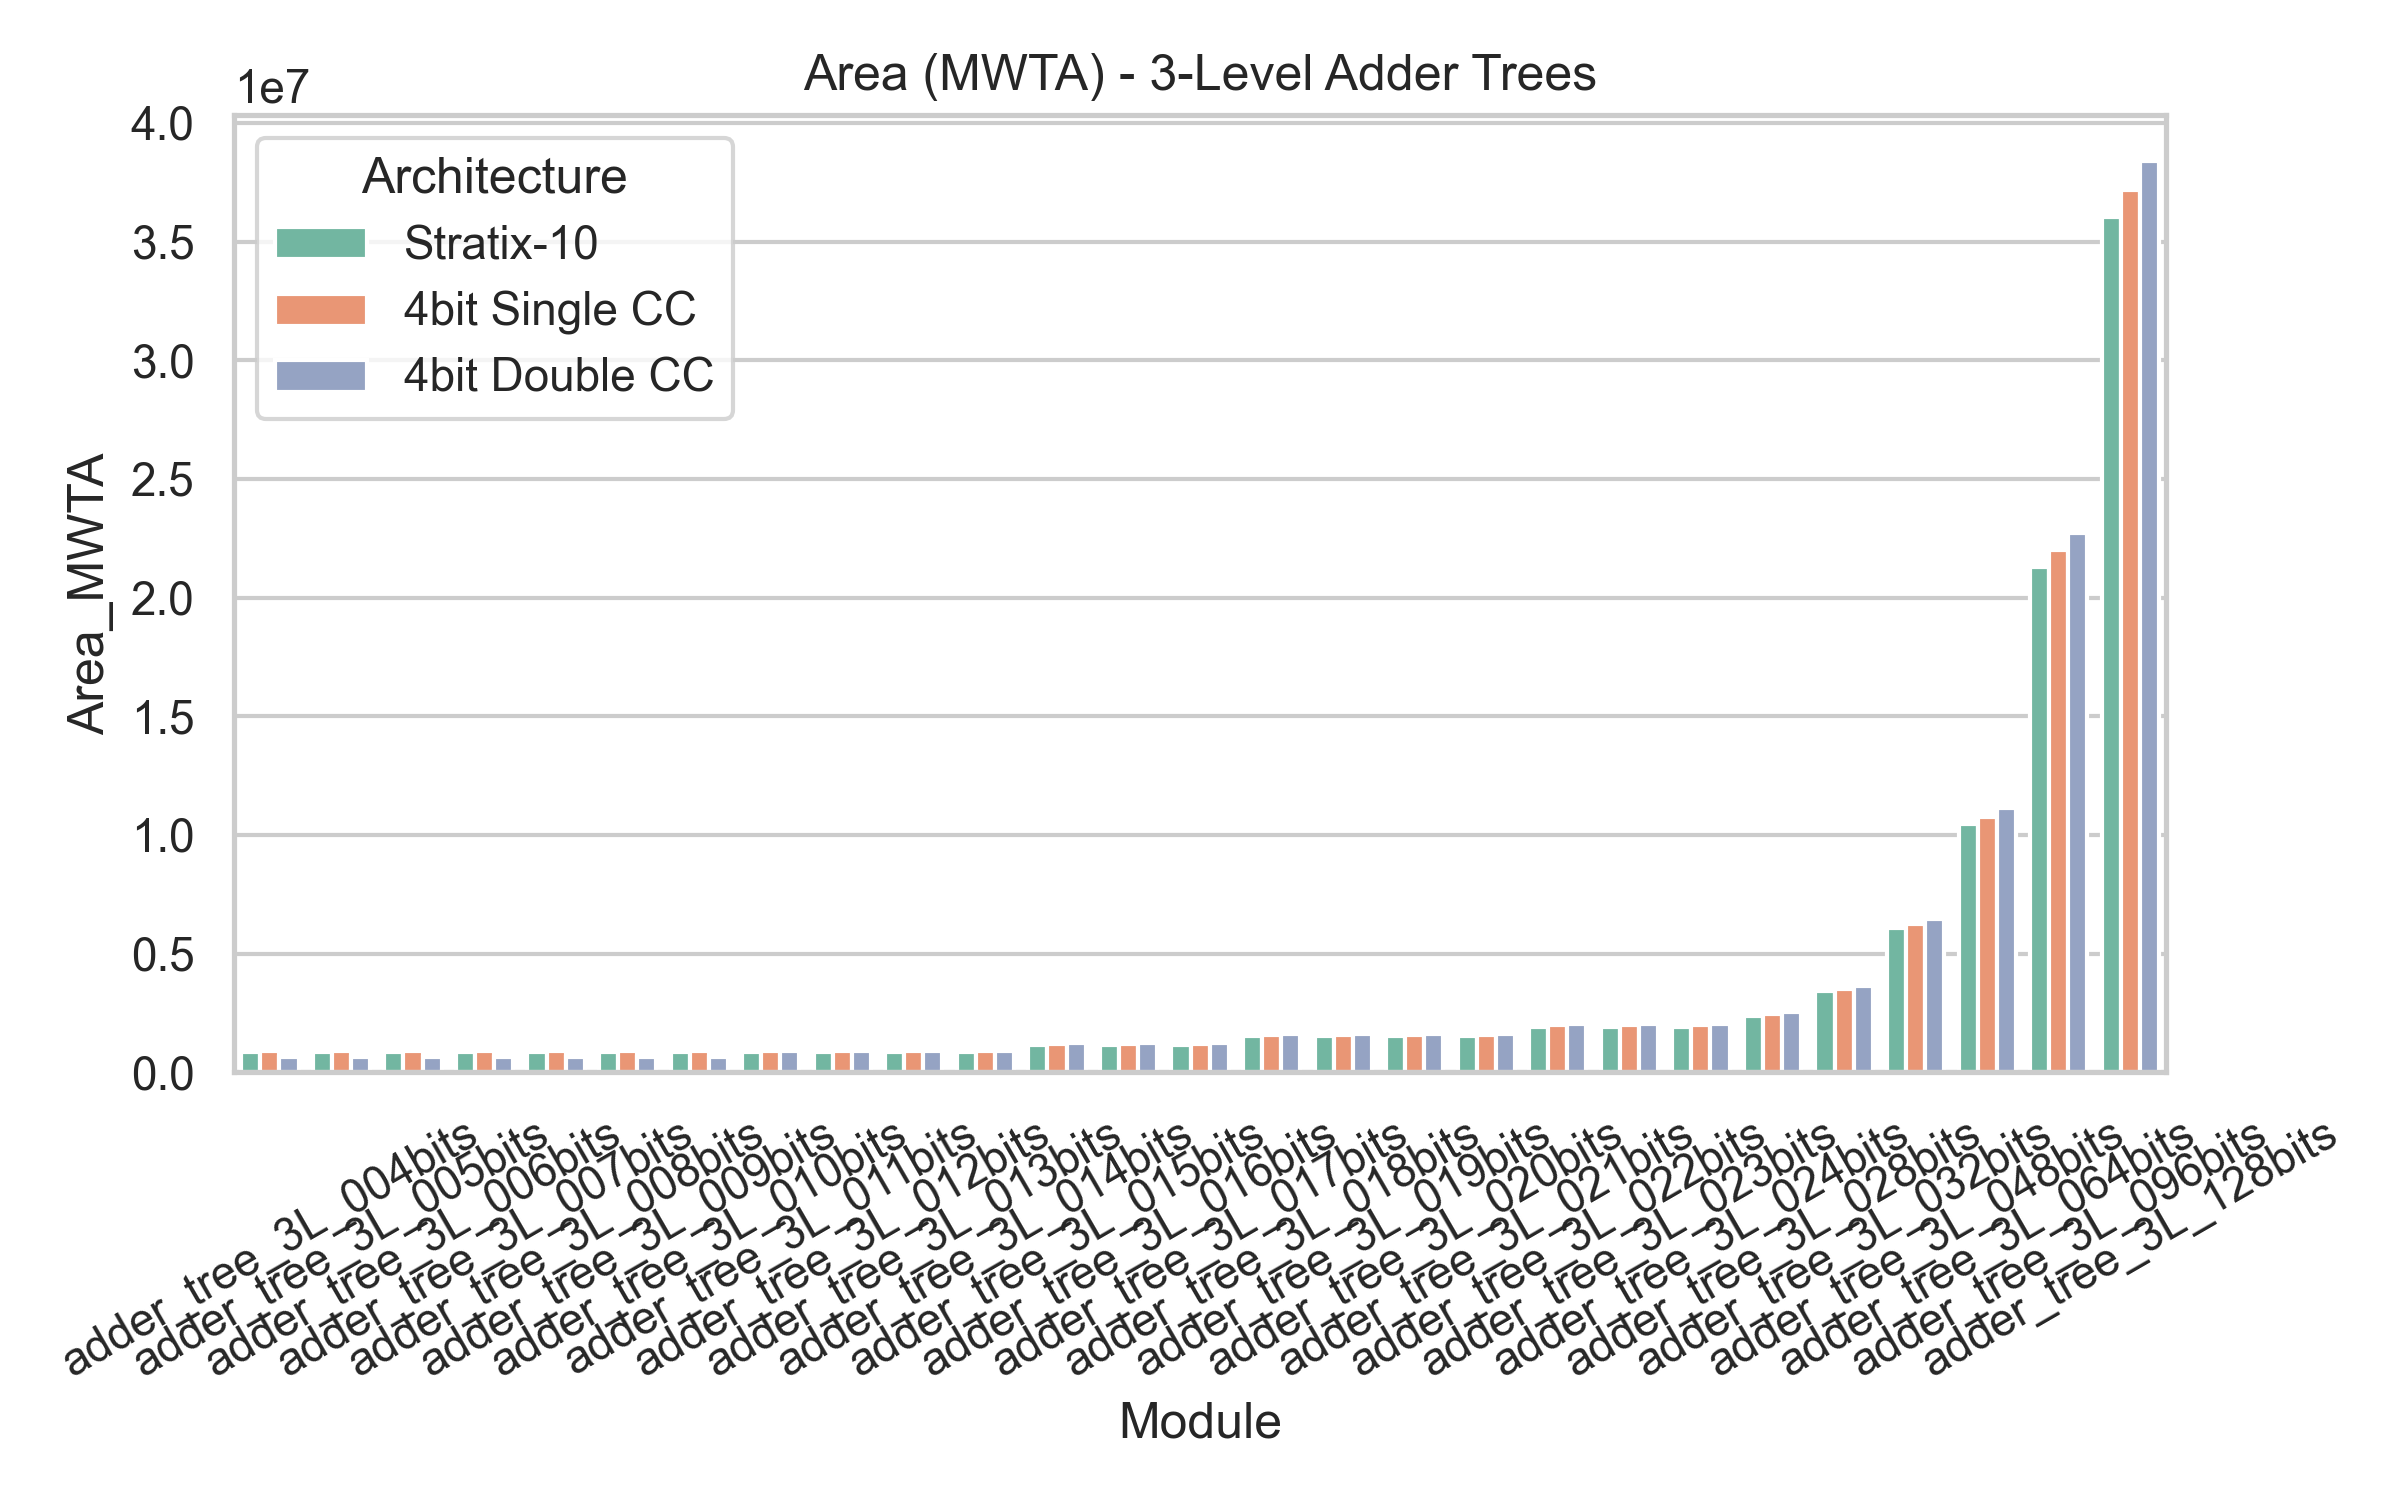
\includegraphics[scale = 0.75]{Figures/adder_trees_3lvl_area_bar_plt.png}}
	\caption{Area (MWTA) Consumption of 3-Level Adder Trees across Architectures}
	\label{fig:Area-(MWTA)-Consumption-of-3-Level-Adder-Trees-across-Architectures}
\end{figure}

This observation reinforces the utility of custom, narrow-precision FPGA fabrics for ML-centric arithmetic workloads, where area efficiency and delay optimization often outweigh the need for generalized functionality.

\subsection{Delay vs Area in FIR Filters}
Fig.\ref{fig:Critical Path Delay vs Area (MWTA) for Wallace Tree based FIR Filters} presents a delay vs area scatter plot for pipelined FIR filters implemented with Wallace Tree multipliers. The data reveals distinct performance clusters for each architecture. In lower-area designs (e.g., filters with fewer taps or lower bit-widths), all three architectures demonstrate similarly low delay (~1–2 ns), indicating minimal routing pressure and simple datapaths. However, as complexity increases, Stratix-10 shows tighter delay control for medium-area FIRs, likely due to its optimized DSP and routing fabric.

\begin{figure}[H]
	\centerline{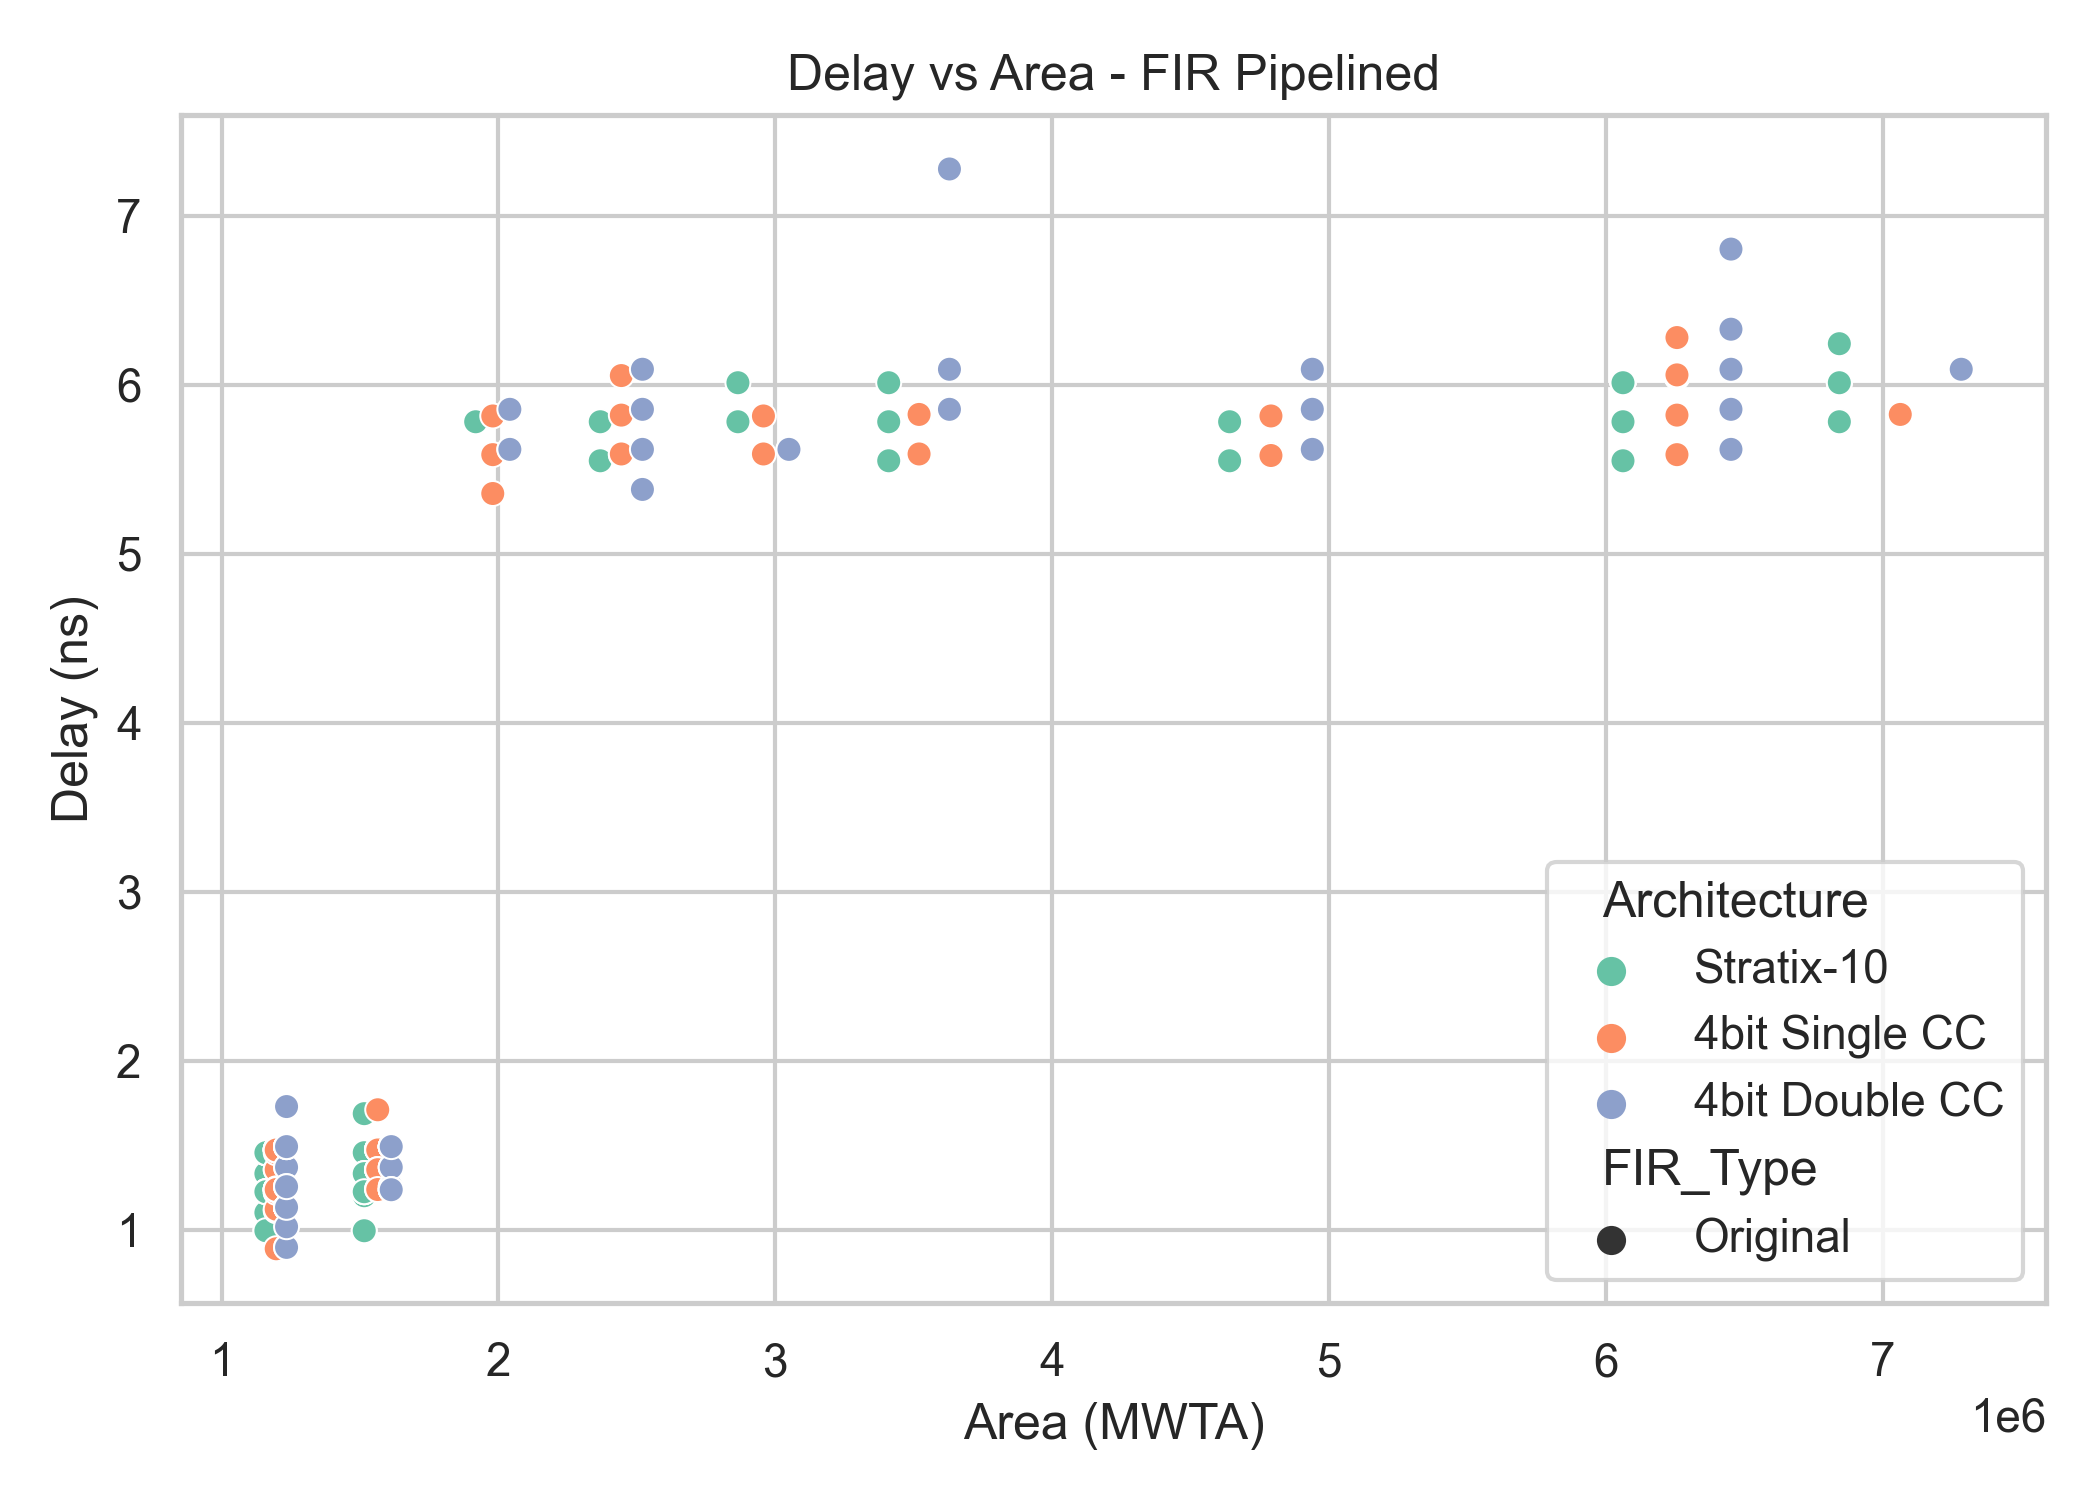
\includegraphics[scale = 0.75]{Figures/fir_pipelined_wallace_delay_area_plt.png}}
	\caption{Critical Path Delay vs Area (MWTA) for Wallace Tree based FIR Filters}
	\label{fig:Critical Path Delay vs Area (MWTA) for Wallace Tree based FIR Filters}
\end{figure}

Interestingly, in larger FIR designs, the 4-bit Single Carry Chain often outperforms Stratix-10 in delay, while maintaining area efficiency. The Double Carry Chain generally uses more area but occasionally yields better delay, reflecting its architectural strength in wide, parallel multiplications. These results demonstrate that specialized carry chain architectures can rival or even surpass commercial FPGAs in delay-area efficiency for structured, low-bitwidth arithmetic pipelines.

\subsection{Delay-Area Product of Unpipelined Wallace Tree based FIR Filters}
The delay-area product analysis of unpipelined FIR filter implementations across three distinct architectures reveals significant performance disparities and scaling characteristics, as shown in Fig.\ref{fig:Delay-Area Product Analysis of Wallace-Tree Unpipelined FIR Filters}.

\begin{figure}[H]
	\centerline{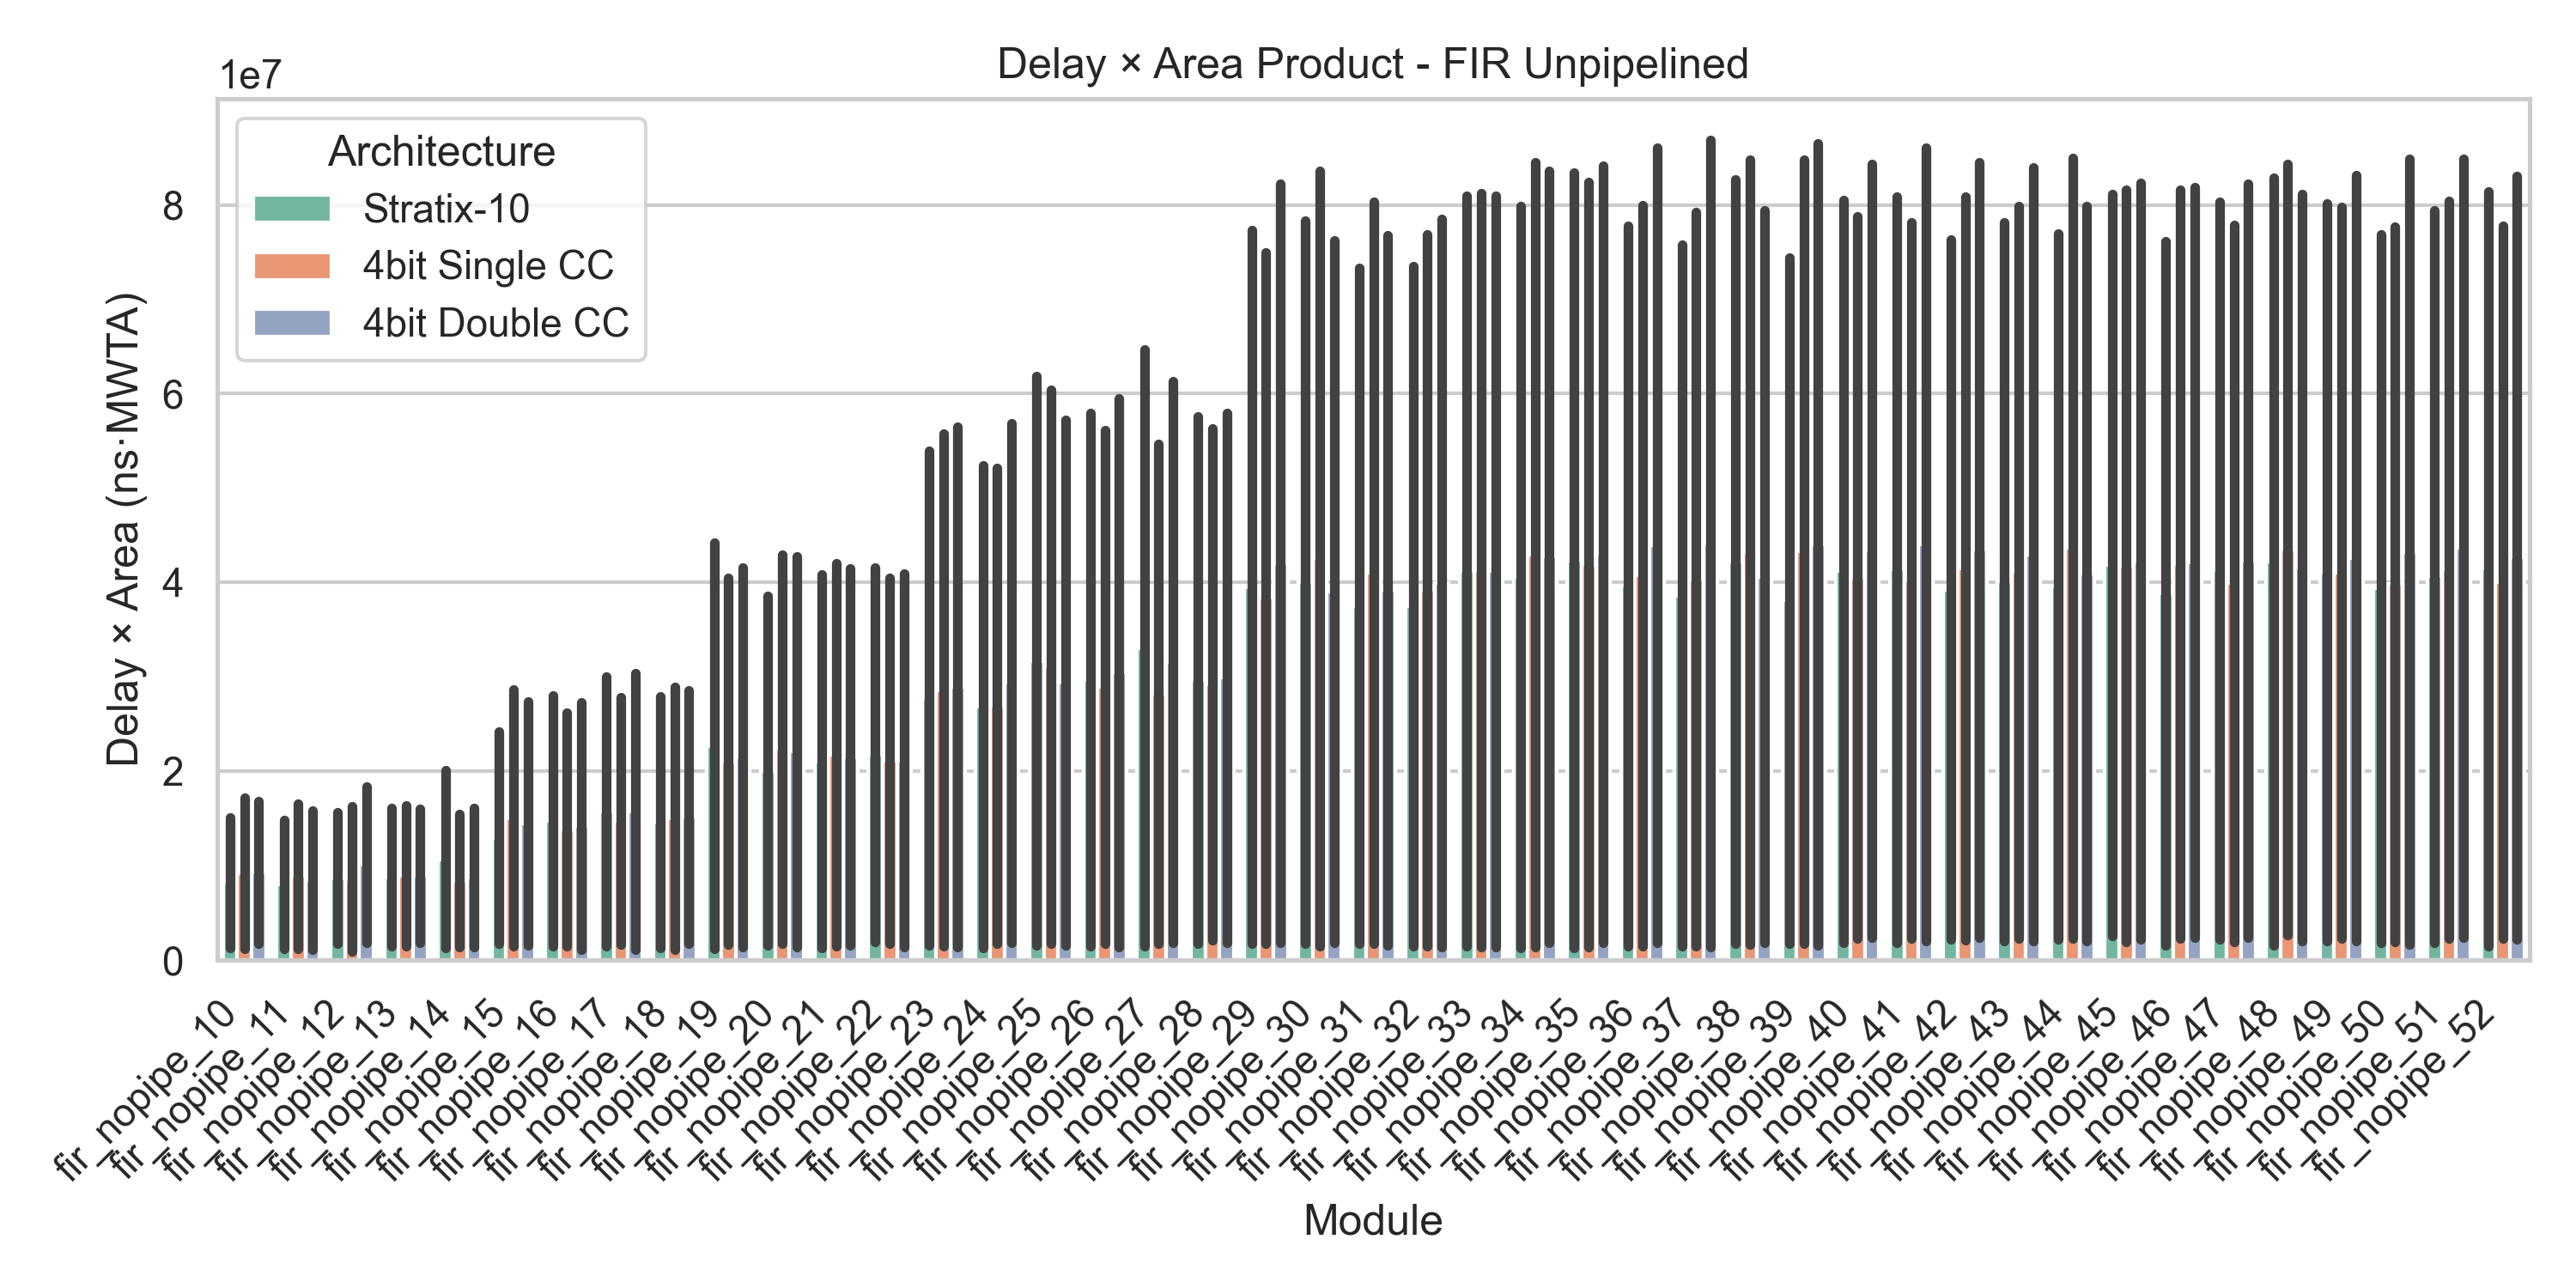
\includegraphics[scale = 0.75]{Figures/fir_unpipelined_wallace_delay_area_prod_plt.png}}
	\caption{Delay-Area Product Analysis of Wallace-Tree Unpipelined FIR Filters}
	\label{fig:Delay-Area Product Analysis of Wallace-Tree Unpipelined FIR Filters}
\end{figure}

The Stratix-10 architecture demonstrates superior efficiency throughout the entire range of filter sizes, consistently achieving the lowest delay-area products with values ranging from approximately 1.5e6 to 8e6 ns·MWTA across modules fir-nopipe-10 through fir-nopipe-52. In contrast, both 4-bit implementations exhibit substantially higher delay-area products, with the 4-bit Single CC architecture showing moderate performance degradation and the 4-bit Double CC architecture displaying the poorest efficiency metrics. All three architectures demonstrate approximately linear scaling behavior with increasing filter complexity, though a notable discontinuity occurs around modules 28-30, suggesting a critical threshold in design complexity. The performance gap between architectures remains relatively constant across different module sizes, with Stratix-10 maintaining approximately 80-90\% lower delay-area products compared to the 4-bit implementations. These results indicate that for unpipelined FIR filter applications, the Stratix-10 FPGA architecture provides substantially better area-delay efficiency, while the 4-bit Double CC approach offers no advantage over the Single CC configuration and should be avoided for this class of implementations.

\subsection{Peak Operational Frequency Analysis}
The top 5 operating frequencies achieved across all benchmarks are summarized in Table 5.1. Notably, the highest frequency — 647.22 MHz — is achieved on the 4-bit Double Carry Chain architecture running a pipelined FIR filter with 12 taps. This aligns with expectations, as the pipelined structure limits combinational depth per stage, while the double carry design accelerates propagation. Interestingly, the 4-bit Single Carry Chain outperforms Stratix-10 in three out of the five cases, demonstrating that targeted low-bitwidth arithmetic architectures can be more frequency-efficient than general-purpose high-end FPGAs in certain domains.

\begin{table}[htb]
	\centering
	\fontsize{10}{12}\selectfont
	\caption{Peak Operational Frequencies}
	\label{tab:peak-operational-frequencies}
	\begin{tabular}{|p{3cm}|c|c|c|}
		%\hline
		%\multicolumn{4}{|c|}{Country List} \\
		\hline
		\textbf{Module}& \textbf {4-Bit Double CC} & \textbf {4-Bit Single CC} & \textbf{Stratix-10}\\
		\hline
		fir-nopipe-11 & 609.25 MHz & 545.15 MHz & 553.98 MHz\\\hline
		fir-pipe-14 & 447.12 MHz & 652.84 MHz & 544.12 MHz\\\hline
		fir-pipe-12 & 647.22 MHz & 489.85 MHz & 494.61 MHz\\\hline
		fir-pipe-27 & 576.59 MHz & 493.45 MHz & 544.12 MHz\\\hline
		fir-pipe-10 & 530.43 MHz & 538.97 MHz & 540.52 MHz\\\hline
		\end{tabular}
\end{table}

These frequency results reinforce the architectural trade-offs: while Stratix-10 offers predictable performance across a wide range of designs, custom carry chain architectures can be tuned to outperform it in narrow, arithmetic-intensive workloads — particularly when pipelining and bit-width optimization are applied.

\section{FPGA Implementation of Manojavam}
This section presents the performance and resource utilization of the Manojavam PCA accelerator when implemented on a Xilinx Artix-7 XC7A35T FPGA using Vivado 2024.1 ML Edition. We report on post-synthesis and post-implementation metrics including logic utilization (LUTs, FFs, DSPs, and BRAMs), maximum achieved clock frequency, power consumption, and timing slack. These results demonstrate how the RTL design maps onto mid-range FPGA fabric, highlighting throughput, energy efficiency, and timing closure for the whole architecture.

\subsection{Resource Consumption}
The FPGA resource utilization of the Manojavam accelerator, synthesized and implemented on the Artix-7 XC7A35T device, is summarized in Table.\ref{tab:manojavam-resource-consumption}.

\begin{table}[htb]
	\centering
	\fontsize{10}{12}\selectfont
	\caption{Manojavam's Resource Consumption}
	\label{tab:manojavam-resource-consumption}
	\begin{tabular}{|p{3cm}|c|c|c|}
		%\hline
		%\multicolumn{4}{|c|}{Country List} \\
		\hline
		\textbf{Resource}& \textbf {Used} & \textbf {Available} & \textbf{Utilization (\%)}\\
		\hline
		LUT & 9796 & 20800 & 47.10\%\\\hline
		FF & 23077 & 41600 & 55.47\%\\\hline
		BRAM & 30.5 & 50 & 61.00\%\\\hline
		DSP & 64 & 90 & 71.11\%\\\hline
	\end{tabular}
\end{table}

This resource profile reflects the architectural demands of Manojavam, which integrates multiple compute-intensive and memory-aware subsystems. The LUT and flip-flop usage—at approximately 47\% and 55\%, respectively—indicates balanced deployment of logic resources, with sufficient margin available for further modular expansion or integration of debugging logic.

BRAM consumption is moderately high at 61\%, consistent with the design’s use of L1 private and shared caches, staging buffers, and operand tile storage for block streaming. This level of memory usage validates the effectiveness of the memory hierarchy and suggests that the accelerator makes full use of the available on-chip memory without exhausting it.

The most saturated resource is the DSP slice count, with 71.11\% of the available multipliers in use. This is directly attributed to the matrix multiplication engine and its 8 systolic arrays, each employing DSP-based MAC units for dense arithmetic. The relatively high DSP usage is a strong indicator that the design is compute-dense and optimized for throughput, making full use of the device's parallel arithmetic capabilities.

In summary, Manojavam fits comfortably within the Artix-7 fabric, striking a balance between compute intensity and architectural scalability. The current resource utilization confirms that the design remains extensible while still exercising the FPGA in a realistic deployment scenario.

\subsection{Power Consumption}
The total power consumption of the Manojavam accelerator on the Artix-7 XC7A35T FPGA is measured at 1.271 W, with the power breakdown across various subsystems detailed below:

\begin{table}[htb]
	\centering
	\fontsize{10}{12}\selectfont
	\caption{Manojavam's Power Consumption}
	\label{tab:manojavam-power-consumption}
	\begin{tabular}{|p{3cm}|c|c|}
		%\hline
		%\multicolumn{4}{|c|}{Country List} \\
		\hline
		\textbf{Power Domain}& \textbf {Power (W)} & \textbf {Percentage of Power}\\
		\hline
		Clocks & 0.036 & 2.83\%\\\hline
		Signals & 0.051 & 4.01\%\\\hline
		Logic & 0.037 & 2.91\%\\\hline
		BRAM & 0.001 & 0.08\%\\\hline
		DSP & 0.036 & 2.83\%\\\hline
		I/O & 1.034 & 81.37\%\\\hline
		Total & 1.271 & 100\%\\\hline
	\end{tabular}
\end{table}

The power profile reveals that I/O activity dominates overall power dissipation, accounting for over 81\% of total power. This is expected, as the design involves continuous tile streaming and operand transfers between the host and the accelerator through external interfaces. Such communication-intensive behavior is inherent to block-streaming architectures, especially when external data sources and sinks are involved.

The internal logic, clocking network, and DSP slices each consume less than 3\% of total power, which highlights the energy efficiency of the compute core. Notably, the DSP slice power (0.036 W) is remarkably low considering that 71\% of DSPs are active, suggesting that the systolic MAC units are operating with low switching activity or short critical paths—benefiting from pipelined execution and localized operand reuse.

Memory power (BRAM) is almost negligible at 0.001 W, which indicates that the cache hierarchy is well-localized and not incurring excessive access toggling. This aligns with the design’s emphasis on temporal locality, where operand tiles are reused before being written back, minimizing memory energy per operation.

The low dynamic power across logic, signal, and clock networks further reinforces that the architecture is streamlined and well-pipelined, with minimal unnecessary toggling. Overall, these figures demonstrate that Manojavam is compute-efficient and memory-efficient, with the majority of power attributed to I/O, which could be optimized in future iterations through embedded memory, DMA interfaces, or tighter system integration.

In summary, Manojavam exhibits a high-performance yet power-conscious architecture, where internal compute blocks operate with minimal overhead, and the primary power bottleneck stems from external communication—an expected but optimizable characteristic in FPGA deployments.

\subsection{Timing Report and Summaries}
The FPGA implementation of Manojavam achieved a maximum operational frequency of 200 MHz after placement and routing on the Artix-7 XC7A35T FPGA. This clock rate reflects the ability of the design to maintain high-throughput performance while satisfying strict timing constraints across the datapath, control, and memory subsystems.

The post-implementation timing analysis yielded the following key results, displayed in Table.\ref{tab:manojavam-timing-report}.

\begin{table}[htb]
	\centering
	\fontsize{10}{12}\selectfont
	\caption{Manojavam's Timing Report}
	\label{tab:manojavam-timing-report}
	\begin{tabular}{|p{3cm}|c|}
		%\hline
		%\multicolumn{4}{|c|}{Country List} \\
		\hline
		\textbf{Timing Metric}& \textbf {Value}\\
		\hline
		Operational Frequency & 200 MHz\\\hline
		Worst Negative Slack (WNS) & 0.203 ns\\\hline
		Worst Hold Slack (WHS) & 0.105 ns\\\hline
		Worst Pulse Width Slack (WPWS) & 1.250 ns\\\hline
	\end{tabular}
\end{table} 

The Worst Negative Slack (WNS) of 0.203 ns indicates that the critical paths in the design meet timing with a narrow but acceptable margin. This confirms that the design is operating within the safe frequency envelope dictated by its longest combinational delay paths. The Worst Hold Slack of 0.105 ns also confirms that short-path timing constraints are met, preventing hold violations and ensuring reliable data transfer between pipeline stages.

A Worst Pulse Width Slack of 1.250 ns further validates that clock signals maintain proper pulse widths, ensuring stable triggering of sequential elements throughout the design. These results, taken together, demonstrate that the Manojavam accelerator closes timing at 200 MHz, with headroom to account for minor PVT (process, voltage, temperature) variations.

The ability to achieve this clock rate on a mid-range FPGA, while also supporting a complex systolic matrix engine and hierarchical memory system, highlights the architectural regularity and timing-friendly layout of the design.

\subsection{Accelerator Floorplanning}
The physical floorplanning of Manojavam on the Artix-7 FPGA played a critical role in achieving its high operational frequency and low power consumption. All major subsystems of the accelerator—namely the 8 systolic arrays, cache hierarchy, controller hierarchy, and the Jacobian unit—were carefully positioned in proximity to the modules they interact with most heavily. This strategic placement minimized routing congestion and reduced signal delays across high-activity interconnects.

The floorplan was not left to automatic placement alone; instead, manual partitioning and logic grouping were applied to tightly cluster compute and memory blocks, enabling highly localized data movement. For instance, each systolic array was physically adjacent to its associated private cache and accumulator, while the shared LHS cache was placed centrally for low-latency broadcasting. This layout was instrumental in supporting efficient pipelined streaming, fast operand reuse, and precise timing closure across the entire design.

To the best of our knowledge, Manojavam is the first PCA accelerator to be floorplanned and deployed with such architectural precision, especially on a mid-range FPGA. This meticulous approach directly contributed to the accelerator’s 200 MHz operational frequency and 1.2 W power envelope—metrics that outperform prior art, which often suffer from thermal bottlenecks or timing failure due to unoptimized physical layouts.

\begin{figure}[H]
	\centerline{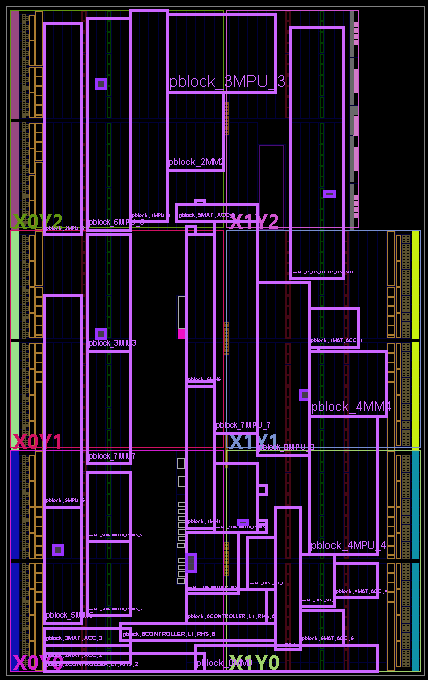
\includegraphics[scale = 1]{Figures/fpga_floorplaned.png}}
	\caption{FPGA Floorplanning of Manojavam}
	\label{fig:FPGA Floorplanning of Manojavam}
\end{figure}

The floorplan layout, shown in Fig.\ref{fig:FPGA Floorplanning of Manojavam}, visually demonstrates the regularity and modularity of the accelerator, further validating the architectural clarity and physical design discipline of the Manojavam system.

\subsection{Comparative Runtime Analysis of PCA on CPU, GPU, and Manojavam Accelerator}
To evaluate the practical benefits of Manojavam in a real-world PCA pipeline, synthetic datasets of dimension $1000xD$, where $D \in {4, 8, 16, 32, 64, 128, 256, 512, 1024}$, were generated using Python. Each dataset was processed through two key stages of the PCA pipeline: matrix multiplication (MM) to compute the covariance matrix, and singular value decomposition (SVD) for eigendecomposition. Execution time for both stages was recorded over 30 independent trials for three platforms:
\begin{enumerate}
	\item CPU : Intel Core i7\cite{chap5-1}
	\item Nvidia A100 (Ampere Architecture)\cite{chap5-2}
	\item Manojavam Accelerator
\end{enumerate}

The average runtime of each stage was recorded, and the total PCA runtime (MM + SVD) was computed. Results were visualized using line plots on logarithmic x-scales to highlight trends across increasing dimensionality.

\subsubsection{Matrix Multiplication (MM) Comparison}
In the MM runtime plot, as shown in Fig.\ref{fig:Execution Time Analysis for Matrix Multiplication}, the Manojavam accelerator shows a consistent linear increase as the feature dimensionality grows, which appears as a straight upward-sloping line on the log-scale graph. This is expected given the tiled 4×4 matrix multiplication strategy with fixed hardware resources and streaming operands. In contrast, both CPU and GPU exhibit nearly flat trends, indicating negligible increases in runtime even as dimensions grow.

\begin{figure}[H]
	\centerline{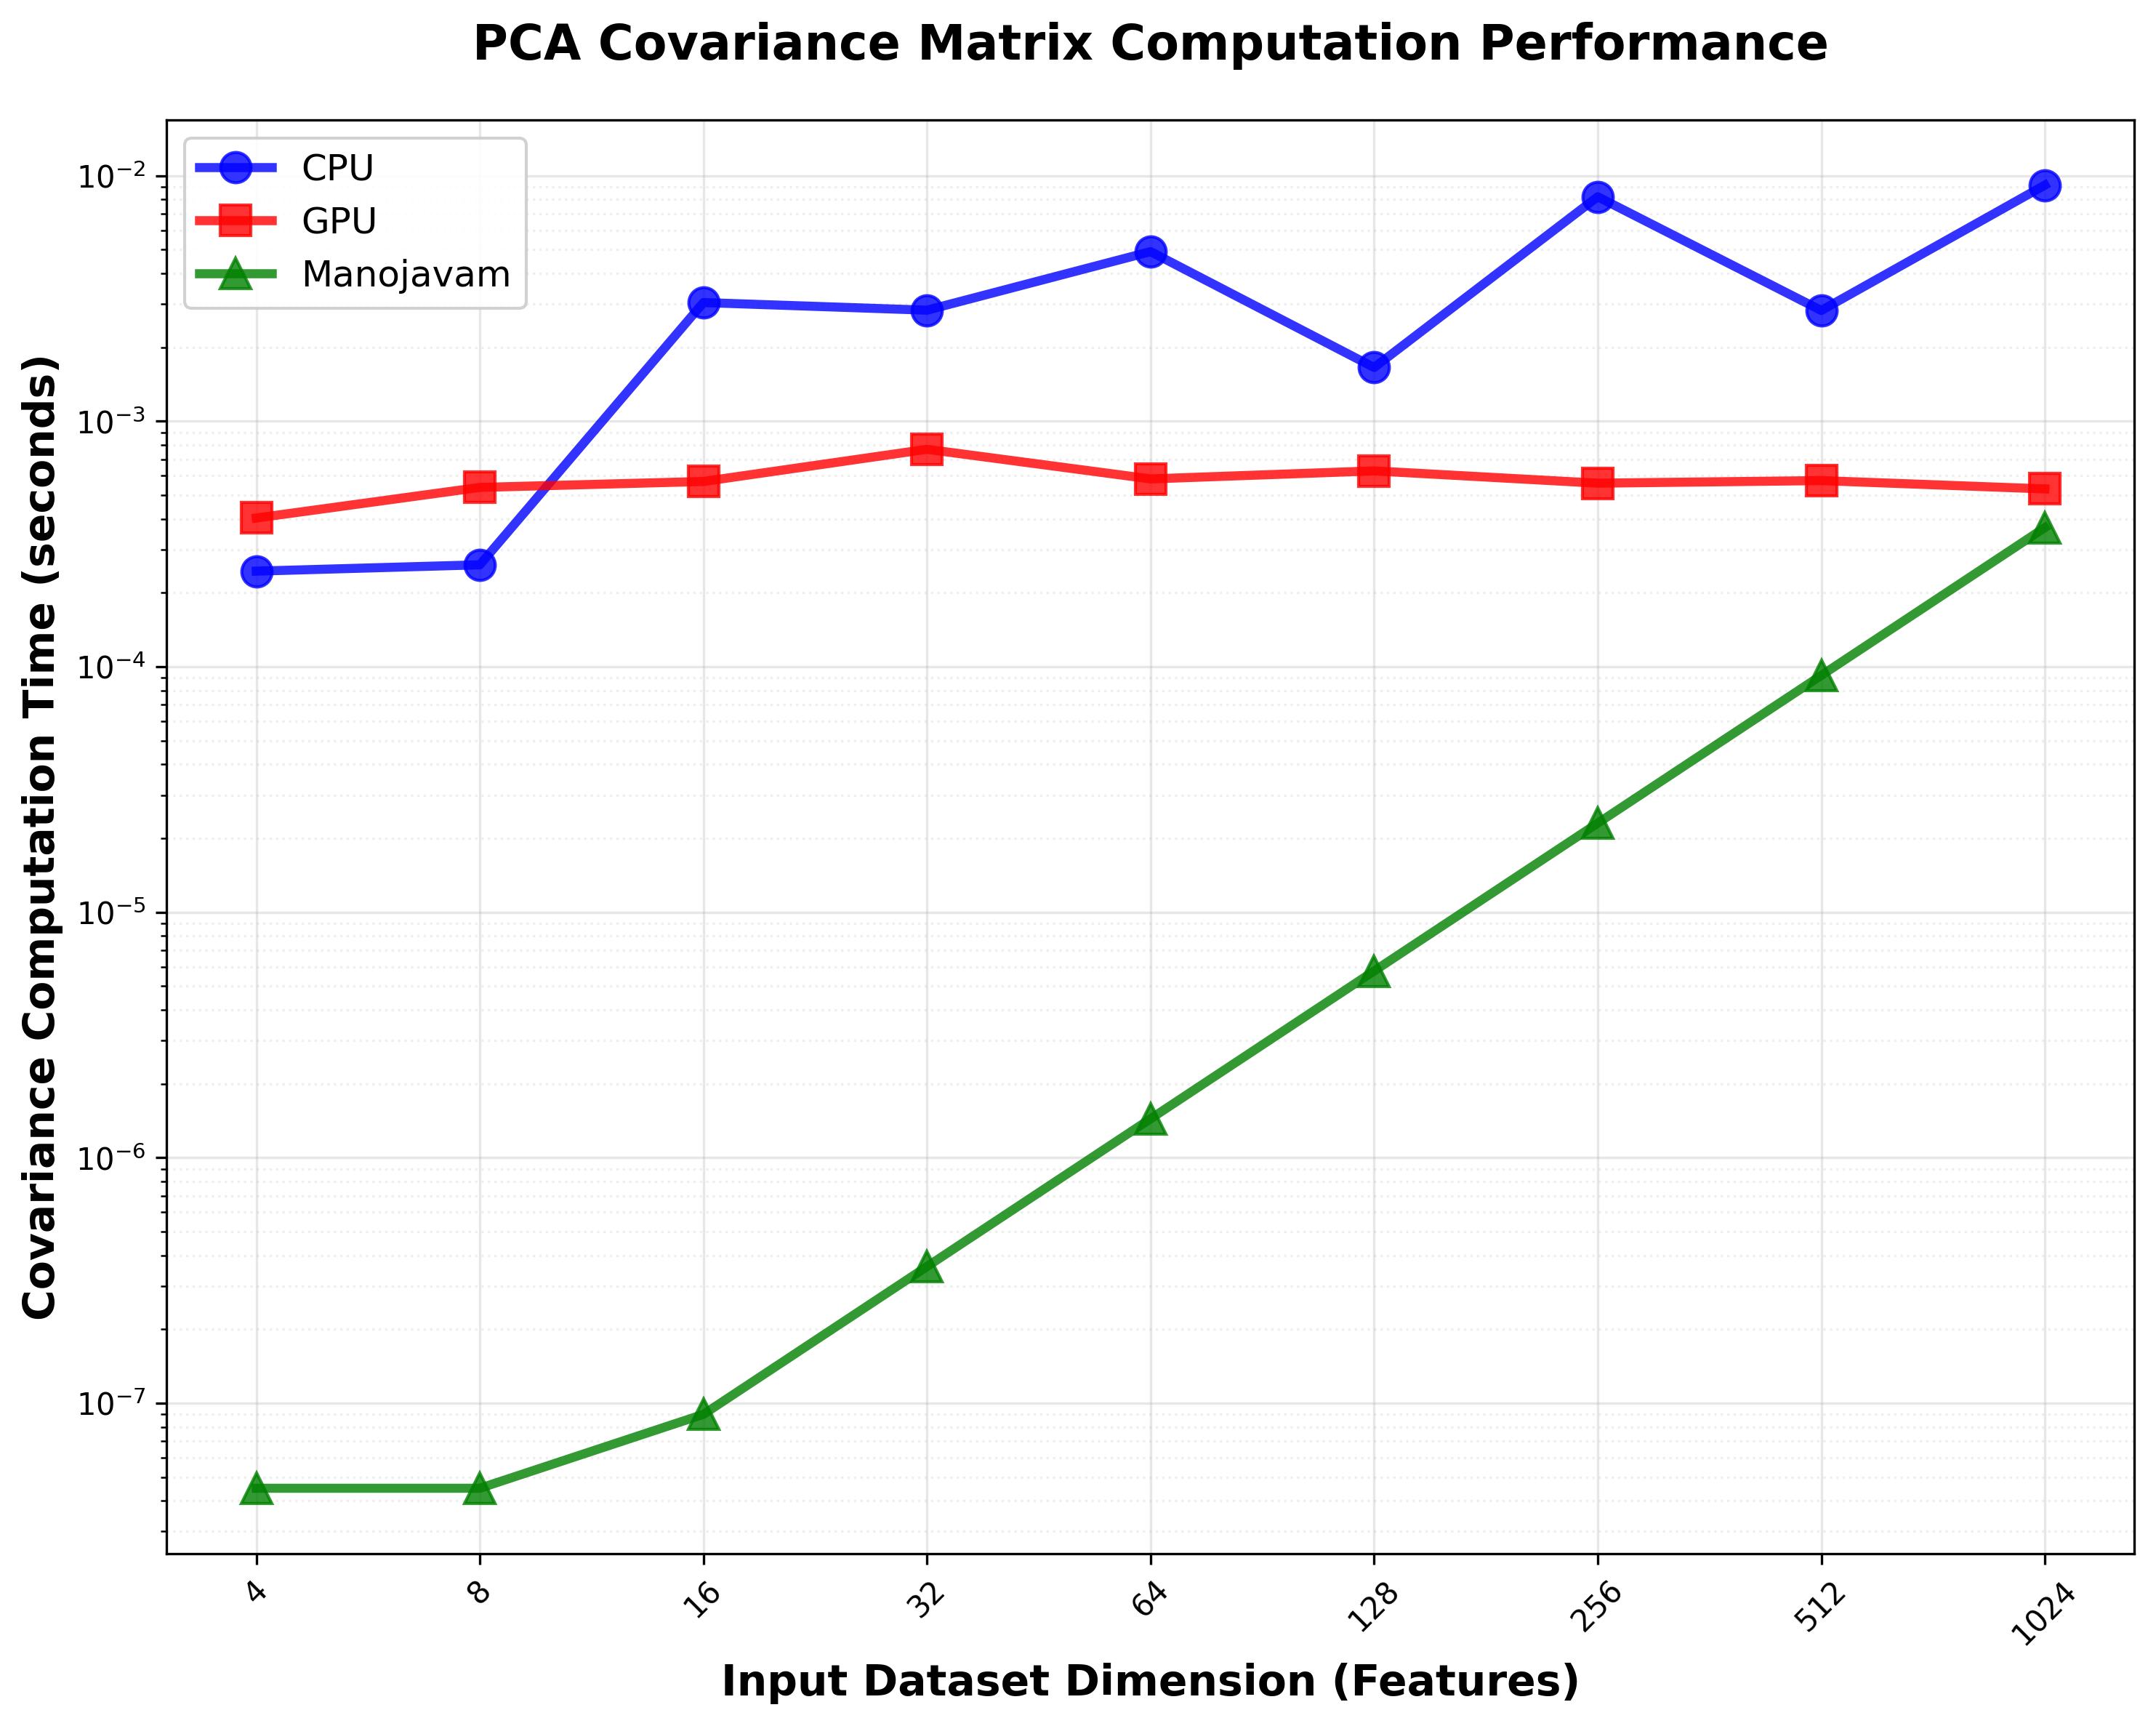
\includegraphics[scale = 0.50]{Figures/covariance_performance.png}}
	\caption{Execution Time Analysis for Matrix Multiplication}
	\label{fig:Execution Time Analysis for Matrix Multiplication}
\end{figure}

This flat trend is due to the use of highly optimized BLAS-backed matrix multiplication libraries (e.g., NumPy on MKL for CPU and cuBLAS for GPU), which leverage massive parallelism, hardware-level acceleration, and cache reuse. While Manojavam does not outperform the CPU or GPU in raw MM runtime, the predictable scaling behavior of its MM engine reflects hardware-deterministic execution, useful in real-time or bounded-latency systems.

\subsubsection{Singular Value Decomposition (SVD) Comparison}
In the SVD runtime plot, all three platforms show linear growth trends with dimensionality, indicating similar algorithmic complexity. However, the Manojavam accelerator consistently achieves the lowest SVD runtime, followed by the GPU, and then the CPU. This ordering holds across all dataset sizes.

\begin{figure}[H]
	\centerline{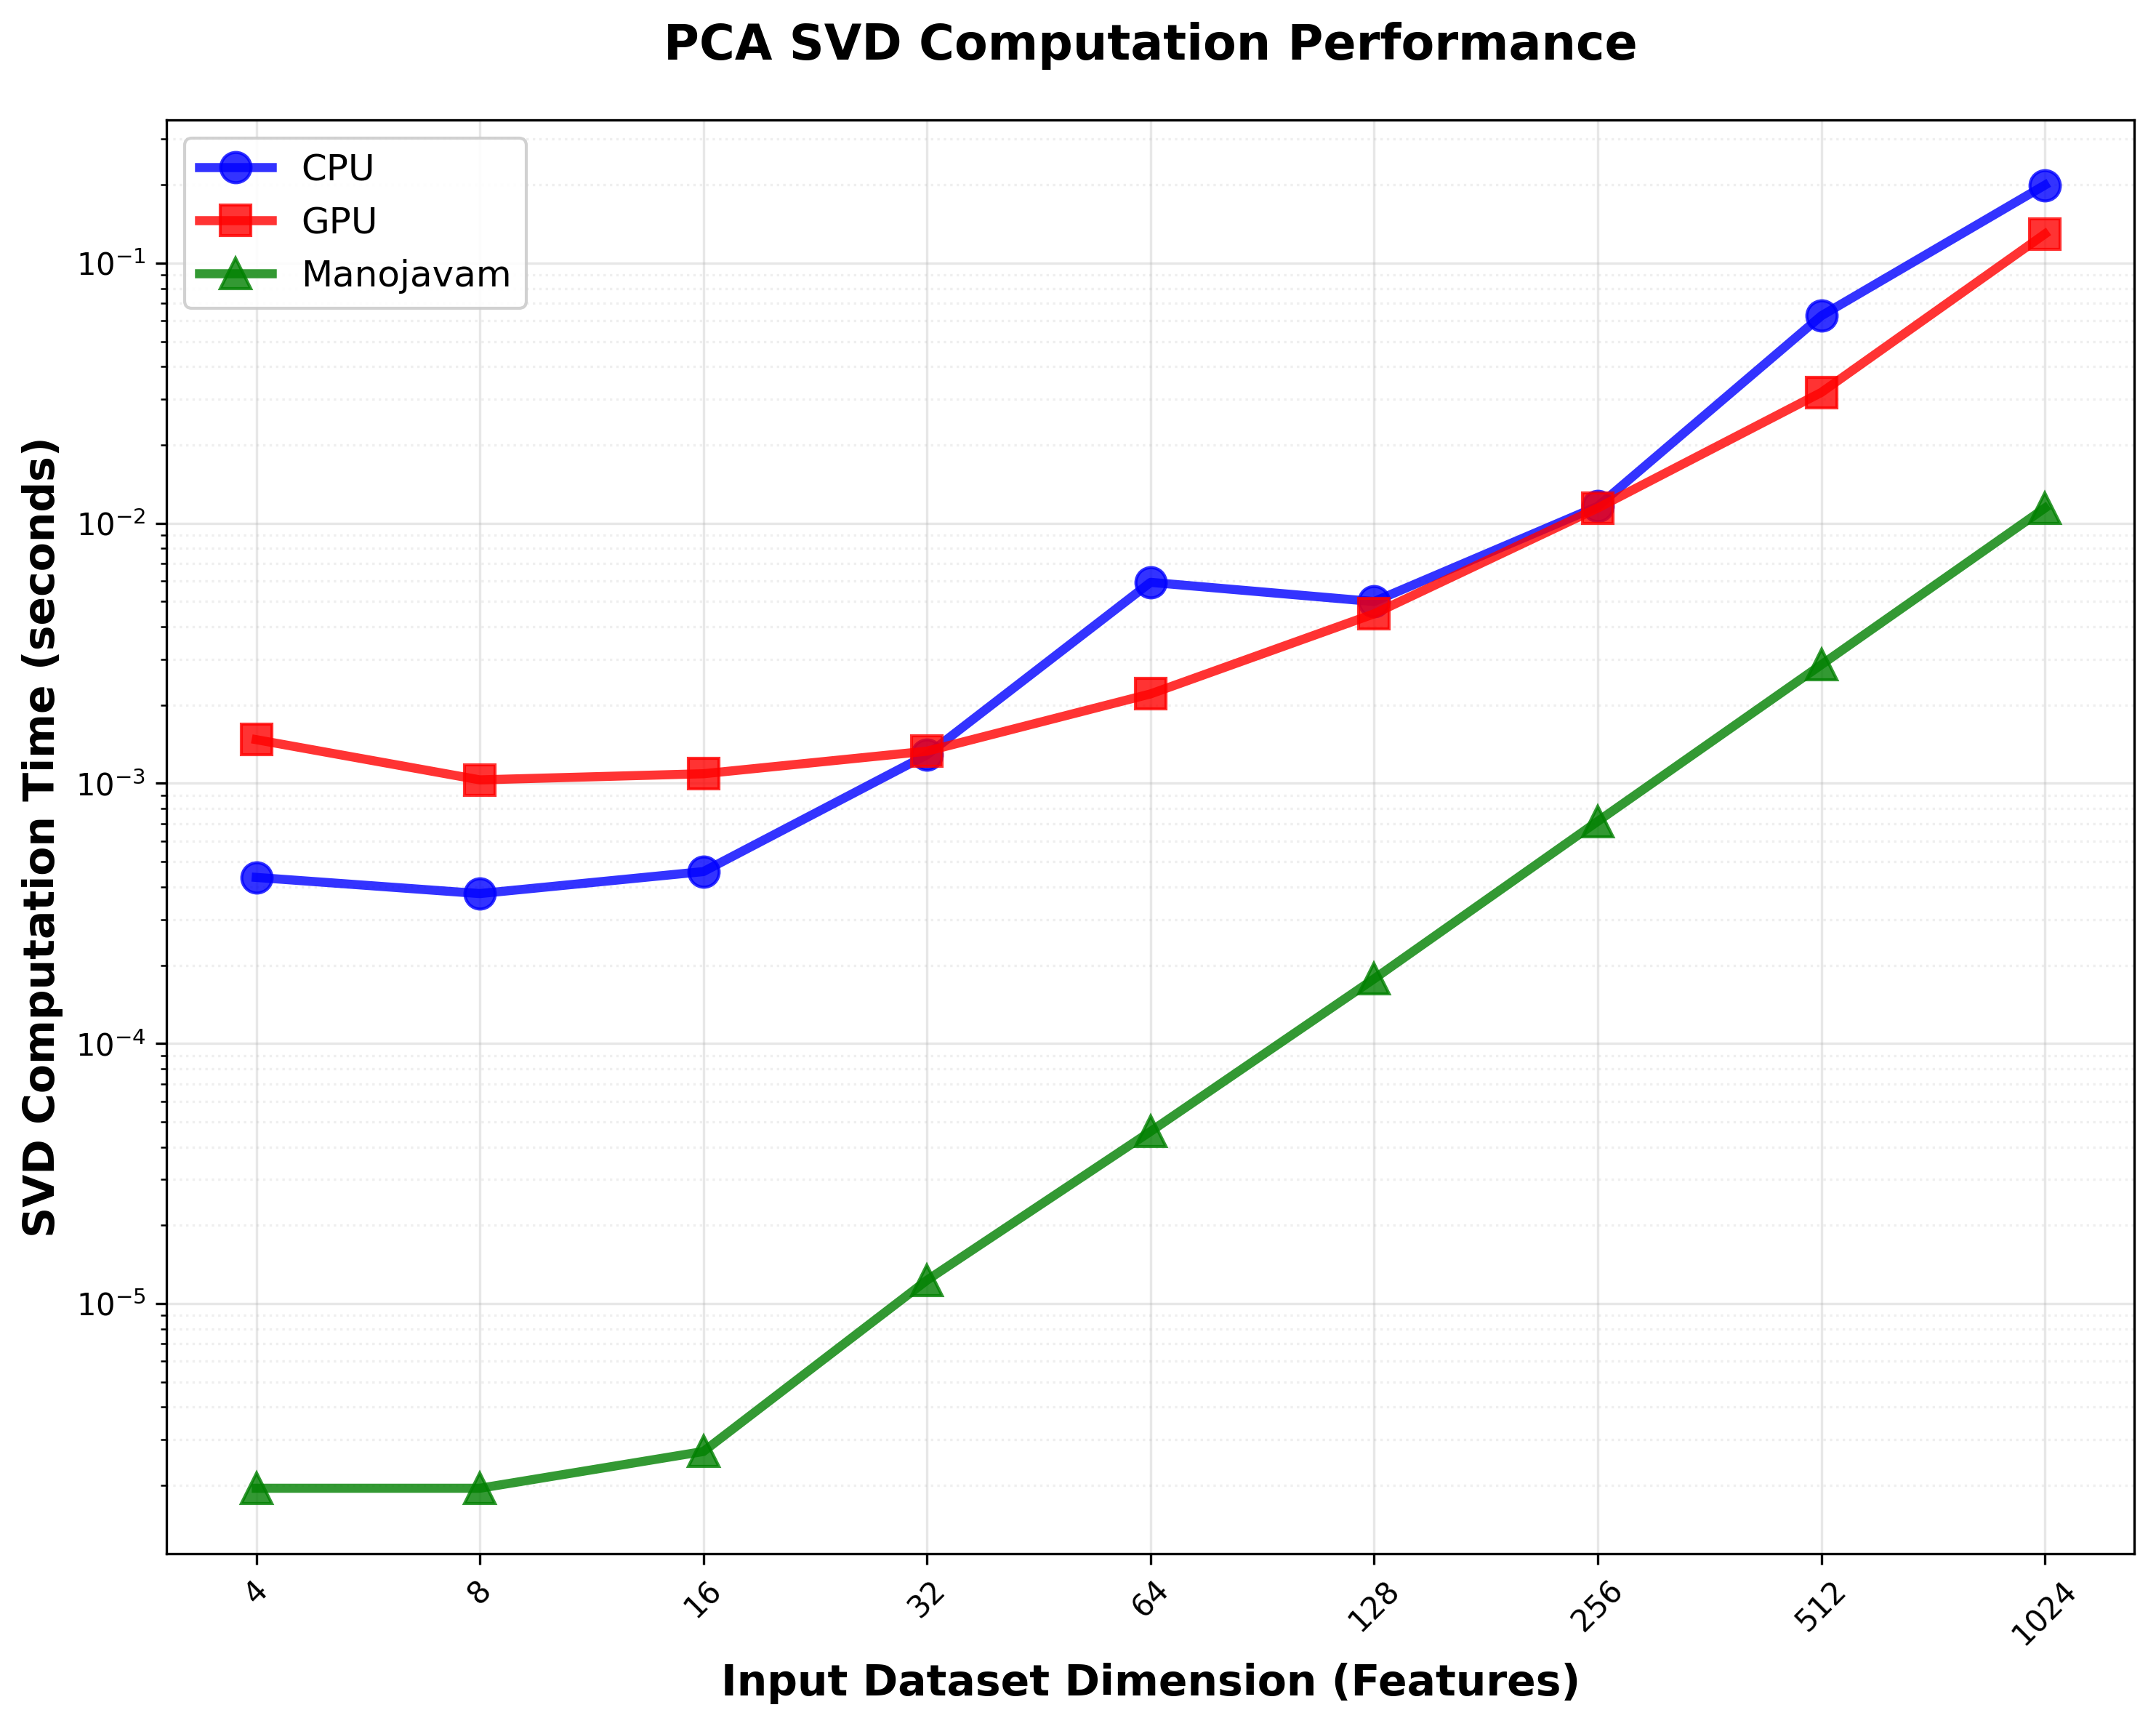
\includegraphics[scale = 0.50]{Figures/svd_performance.png}}
	\caption{Execution Time Analysis for Singular Value Decomposition}
	\label{fig:Execution Time Analysis for Singular Value Decomposition}
\end{figure}

This result is particularly notable because SVD is often considered a memory-bound operation involving iterative rotations or decomposition steps. Manojavam's hardware-level implementation of the Jacobi method using custom control and rotation logic enables this advantage. The locality of operand tiles, tight scheduling, and fixed datapath precision reduce both memory latency and compute overhead, allowing Manojavam to outperform even the highly optimized A100 GPU.

\subsubsection{Total Runtime Comparison (MM + SVD)}
In the total runtime plot, all three platforms show increasing trends across the log-scale x-axis, as expected. However, due to its superior SVD performance, the total execution time for Manojavam remains consistently lower than both GPU and CPU across all dataset sizes.

\begin{figure}[H]
	\centerline{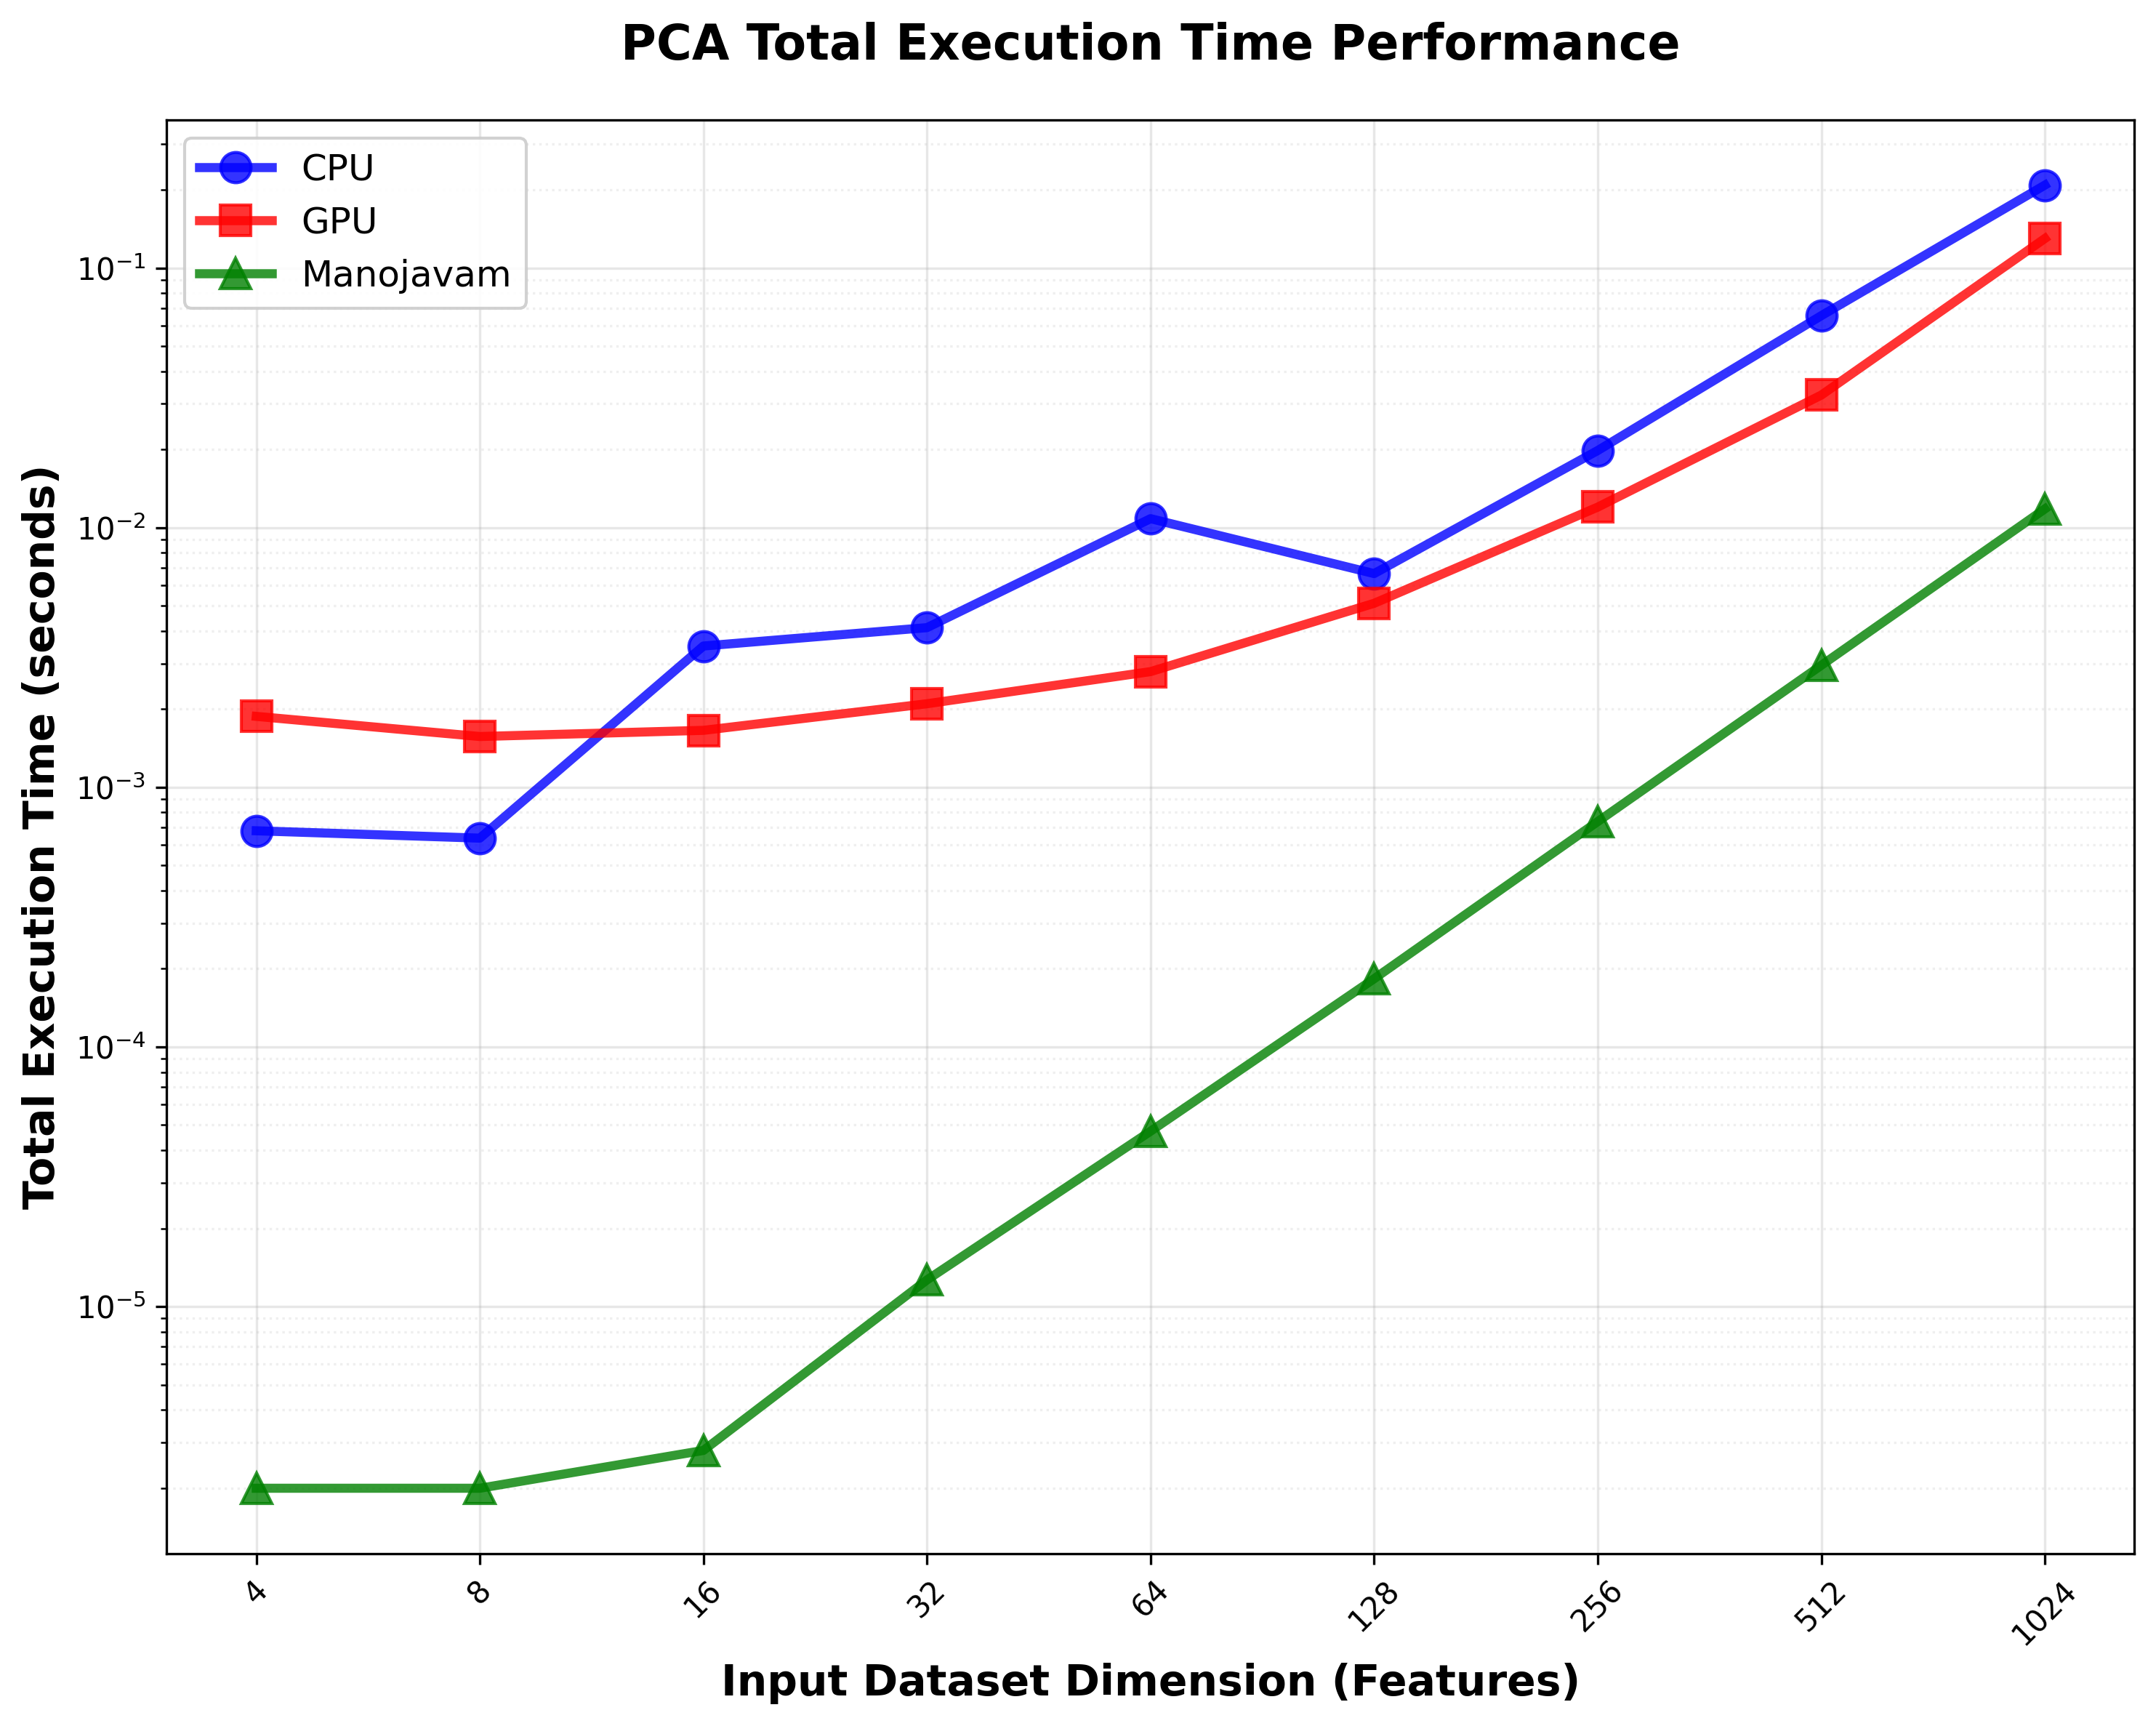
\includegraphics[scale = 0.50]{Figures/total_performance.png}}
	\caption{Total Execution Time Analysis}
	\label{fig:Total Execution Time Analysis}
\end{figure}

While the matrix multiplication stage is not the fastest, its contribution is amortized by the highly efficient SVD pipeline. The GPU consistently outperforms the CPU, but neither platform is able to match the hardware-convergent execution pattern of Manojavam. This demonstrates the benefit of accelerator specialization, where targeted architectural decisions (e.g., streaming memory, pipelined Givens rotations) can lead to substantial end-to-end speedups even against massively parallel general-purpose hardware.

\subsubsection{Detailed Performance Analysis}
To assess the performance characteristics of Manojavam in depth, detailed timing measurements were recorded for each stage of the PCA pipeline—covariance matrix computation and singular value decomposition (SVD)—at increasing feature dimensionalities, ranging from 4 to 1024. Execution times for the CPU (Intel Core i7), GPU (NVIDIA A100), and the Manojavam accelerator were recorded and averaged across 30 trials per configuration.

At a feature size of 1024—representative of high-dimensional PCA workloads—Manojavam exhibits substantial performance advantages over both CPU and GPU implementations. The following speedups were recorded:

\begin{itemize}
	\item \textbf{Covariance Matrix Computation}
	\begin{enumerate}
		\item \textbf{25x} faster than CPU
		\item \textbf{1x} faster than GPU (on par with GPU)
	\end{enumerate}
	\item \textbf{SVD Computation}
	\begin{enumerate}
		\item \textbf{17x} faster than CPU
		\item \textbf{11.3x} faster than GPU
	\end{enumerate}
	\item \textbf{Total PCA Runtime}
	\begin{enumerate}
		\item \textbf{18x} faster than CPU
		\item \textbf{11x} faster than GPU
	\end{enumerate}
\end{itemize}

These results underscore the hardware-level efficiency of Manojavam's design. While matrix multiplication is a well-optimized primitive on both CPUs and GPUs (especially with libraries like MKL and cuBLAS), Manojavam remains competitive due to its pipelined, tile-streamed systolic engine. The real breakthrough, however, comes from the SVD stage, where the custom-built Jacobi unit dramatically outperforms both software platforms by exploiting data locality, reduced precision, and deterministic execution.

\section{ASIC Implementation of Manojavam}
Here we quantify the ASIC implementation of Manojavam using the OpenLane flow with integrated OpenRAM macros. Key metrics include synthesized gate-level area, floorplanned core utilization, post-route timing (worst negative slack, achievable clock frequency), power estimates (dynamic and leakage), and signoff validation (DRC/LVS). These results illustrate the accelerator’s silicon footprint, timing performance, and power profile in a process-technology context, providing a direct comparison to the FPGA implementation and validating the design’s readiness for custom silicon deployment.

Fig.\ref{fig:manojavam-asic} depicts the GDSII layout of the chip as viewed in OpenRoad's GUI.
\begin{figure}
	\centerline{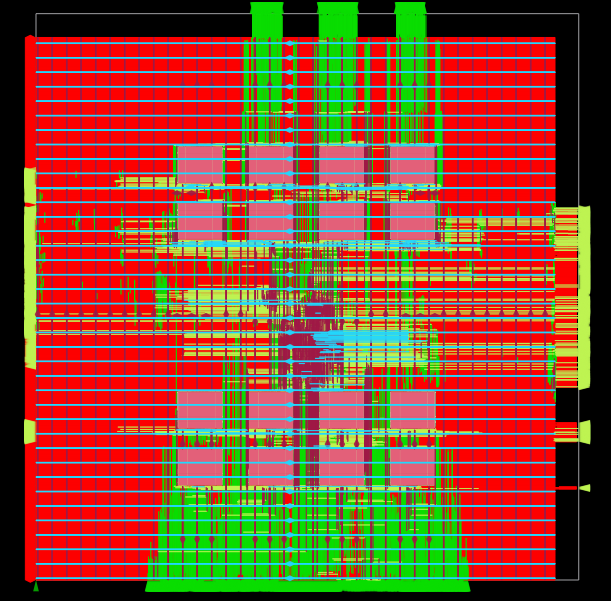
\includegraphics[scale = 0.8]{Figures/manojavam_asic_layout.png}}
	\caption{Manojavam ASIC}
	\label{fig:manojavam-asic}
\end{figure}

\subsection{Synthesis Reports}
The ASIC synthesis of Manojavam was carried out using the OpenLane flow, with Yosys as the front-end logic synthesizer. The design successfully passed through RTL synthesis without the need for memory macros or behavioral process constructs, resulting in a structurally flat, fully synthesizable netlist.

The post-synthesis report shows that a total of 28,816 standard cells were instantiated to implement the full Manojavam accelerator pipeline, including systolic arrays, matrix accumulators, controller hierarchies, and cache logic. A summary of relevant statistics extracted from the synthesis log in Table.X

\begin{table}
	\centering
	\fontsize{10}{12}\selectfont
	\caption{Manojavam-ASIC Resource Utilization}
	\label{tab:manojavam-asic-utilization-report}
	\begin{tabular}{|p{6cm}|c|}
		%\hline
		%\multicolumn{4}{|c|}{Country List} \\
		\hline
		\textbf{Metric}& \textbf {Value}\\
		\hline
		Number of Wires & 37630\\\hline
		Number of wire bits & 40244\\\hline
		Number of public wires & 4136\\\hline
		Number of public wire bits & 6750\\\hline
		Number of processes & 0\\\hline
		Number of memories & 0\\\hline
		Number of cells & 37661\\\hline
	\end{tabular}
\end{table} 

The synthesized design occupies a total core area of approximately 3451742.2592 $\mu m^{2}$, as reported by OpenLane's post-synthesis analysis. The overall layout uses a die-area of 5750 × 6000 $\mu m^{2}$ and a core-area of 5500 × 5750 $\mu m^{2}$, resulting in a core utilization of 50\%. This indicates a healthy placement density, leaving ample white space for routing resources, clock trees, and potential macro additions in future versions.

\subsection{Power Reports}
The power analysis for Manojavam's ASIC implementation was conducted using the OpenLane flow under typical PVT corner conditions, with activity estimation enabled. The total power consumption of the accelerator is reported as 0.154 W (154 mW), which includes contributions from internal switching, signal transitions, and leakage across all logic domains.

A breakdown of power consumption by subsystem is provided in Table.\ref{tab:manojavam-asic-power-report}.
\begin{table}
	\centering
	\fontsize{10}{12}\selectfont
	\caption{Manojavam-ASIC Power Report}
	\label{tab:manojavam-asic-power-report}
	\begin{tabular}{|p{3cm}|c|c|c|c|c|}
		%\hline
		%\multicolumn{4}{|c|}{Country List} \\
		\hline
		\textbf{Power Group} & \textbf {Internal (W)} & \textbf {Switching (W)} & \textbf {Leakage (W)} & \textbf {Total Power (W)} & \textbf {\% of Total}\\
		\hline
		Sequential Logic & 0.0219 & 0.00498 & 3.92e-08 & 0.0269 & 17.5\%\\\hline
		Combinational Logic & 0.0360 & 0.0188 & 1.88e-07 & 0.0548 & 35.6\%\\\hline
		Clock Network & 0.00634 & 0.00408 & 3.57e-08 & 0.0104 & 6.8\%\\\hline
		SRAMs & 0.0614 & 0 & 3.05e-04 & 0.0617 & 40.1\%\\\hline
		I/O and Pads & 0 & 0 & 0 & 0 & 0\%\\\hline
		\textbf{Total} & 0.126 & 0.0278 & 0.000305 & 0.154 & 100\%\\\hline
	\end{tabular}
\end{table}

The macro power contribution—comprising 40.1\% of total power—is dominated by the SRAM macros integrated into the accelerator. These macros, used for operand and intermediate tile storage, incur a modest internal power cost but show no switching activity, indicating energy-efficient access patterns and low toggle rates due to spatial data reuse.

Combinational logic, largely attributed to the 8 systolic arrays and controller datapaths, accounts for 35.6\% of total power. This reflects active arithmetic computation but remains within a highly optimized range due to the systolic array's regular structure and local communication pattern.

Sequential elements, including flip-flops in accumulation and control stages, contribute 17.5\% to power, while the clock distribution network contributes only 6.8\%, signaling an efficient and well-buffered CTS stage with limited skew domains.

Leakage power across the entire design is extremely low—just 0.2\% of the total—which is consistent with the synthesized gate-level netlist and the use of typical corner process models.

The power profile of Manojavam demonstrates a high degree of energy efficiency, with over 81\% of the power being dynamic in nature, and the rest evenly split across the clock and macro systems. When paired with the physical floorplan and power density visualization (shown in Figure 5.x), this analysis confirms the thermal viability and low-power operation of the ASIC variant of Manojavam, making it suitable for embedded and edge ML deployments. 

\subsection{Routing Results}
The routing phase of Manojavam's ASIC implementation completed successfully using the OpenLane flow, with full connectivity achieved across all signal nets and macros. The design passed detailed routing with zero DRC violations, confirming adherence to the process design rules and ensuring manufacturability.

\begin{figure}
	\centerline{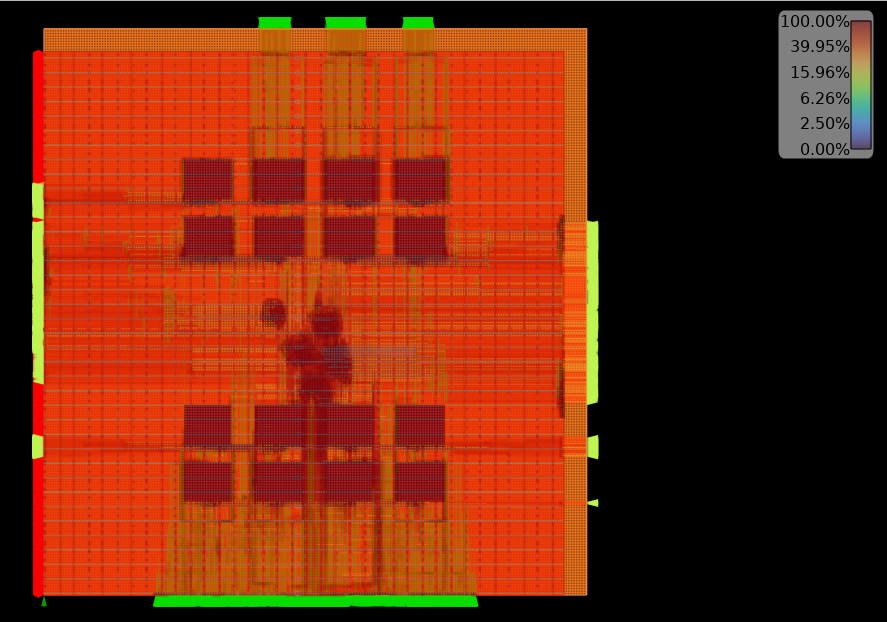
\includegraphics[scale = 0.80]{Figures/routing_layout.png}}
	\caption{Manojavam ASIC Routing Layout View}
	\label{fig:Manojavam ASIC Routing Layout View}
\end{figure}

A routing congestion analysis, visualized in Fig.\ref{fig:Manojavam ASIC Routing Layout View}, reveals that the design maintained a consistent congestion level of approximately 40\% across the core layout. This moderate and uniformly distributed routing density is a positive indicator of balanced floorplanning, optimized placement, and well-structured interconnect design. It suggests that no region of the chip suffers from critical wiring bottlenecks, and the routing tool was able to utilize metal layers efficiently without over-saturating specific areas.

This uniform congestion profile also implies reduced risk of timing degradation and lower power dissipation due to wire capacitance, both of which contribute to the design’s physical and electrical robustness. Overall, the routing stage validates the quality of the design's layout structure and affirms its readiness for GDSII generation and fabrication.

 

\begin{comment}
All the results obtained for your objectives should be discussed in this chapter. This chapter should contain the following sections as per the project.
\begin{enumerate}
\item Simulation results
\item Experimental results
\item Performance Comparison
\item Inferences drawn from the results obtained
\end{enumerate}
All the figures should be properly explained by bringing the scenarios of the design done in the project. A detailed discussion of results obtained should be done in this chapter.

\section{Tables in thesis}
\begin{itemize}
	\item All Table Caption should be in Sentence Case, TNR 10 Pt. It should be of the Format:
	\begin{itemize}
		\item Table 1.1 Results of the experiment ….(Centered)
	\end{itemize}
	\item It should be cited as Table 1.1.
	\item Caption should appear above the Table.
	\item Table Header and the entries should be of Font TNR 10 Pt, Justified.
	\item For wider Table, the page orientation can be Landscape.
	\item For Larger Table, it can run to pages and the header should be repeated for each page of the Table.
	\item Table must be adjusted to fit in the page and no single row is left out for a new page.	
\end{itemize}

Sample Table \ref{c5:tab1} is given below for your reference,

\begin{table}[htb]
\fontsize{10}{12}\selectfont
\caption{Country List}
\label{c5:tab1}
\begin{tabular}{|p{3cm}|c|c|c|}
	%\hline
	%\multicolumn{4}{|c|}{Country List} \\
	\hline
	\textbf{Country Name     or Area Name}& \textbf {ISO ALPHA 2 Code} & \textbf {ISO ALPHA 3 Code} & \textbf{ISO numeric Code}\\
	\hline
	\textbf{Afghanistan}   & AF    & AFG &   004\\\hline
	\textbf{Aland Islands}&   AX  & ALA   & 248\\\hline
	\textbf{Albania} & AL & ALB&  008\\\hline
	\textbf{Algeria}    &DZ & DZA&  012\\\hline
	\textbf{American Samoa}&   AS  & ASM&016\\\hline
	\textbf{Andorra}& AD  & AND   & 020\\\hline
	\textbf{Angola}& AO  & AGO& 024\\
	\hline
\end{tabular}
\end{table}

%\begin{table}[htp]
%\fontsize{10}{12}\selectfont
%\centering
%\caption{Data units, sources, and dates} \label{c5:tab2}
%\begin{tabular}{| *4{>{\arraybackslash}m{1in}|} @{}m{0pt}@{}}
%	\hline
%	\textbf{Variable} & \textbf{Dates} & \textbf{Units} &
%	\textbf{Source}  &\\[2ex] 
%	\hline
%	\textbf{Nominal Physical Capital Stock} & 1950-1990 & Billions
%			US\$ & Nehru and Dhareshwar (1993) &\\[0ex]
%	\hline
%	\textbf{Total Population} & 1950-1990 & Billions & Nehru and
%			Dhareshwar (1993) &\\[0ex]
%	\hline
%	\textbf{Nominal GDP} & 1950-1990 & Billions  US\$ & PWT &\\[5ex]
%	\hline
%	\textbf{Real GDP per capita} & 1950-1990 & 2005 US\$ per capita & PWT &\\[5ex]
%	\hline
%\end{tabular}
%\end{table}

\section{Math equation in thesis}
All equation should be written using equation editor or using an equivalent tool.
\begin{itemize}
	\item Equations should be numbered as : 1.1, 1.2 ...
	\item Equation should be Centered, 12 Pt, TNR. 
	\item Equation number should be right Justified
	\item It should be cited as Eqn. 1.1.
   \item If the sentence starts by citing an equation, then it should be written as Equation 1.1 For example, Equation 5.1 states the Pythagoras theorem.

	
\end{itemize}

For example in Eqn. \ref{c5:eqn1}, The well known Pythagorean theorem $x^2 + y^2 = z^2$ was 
proved to be invalid for other exponents. 
Meaning the next equation has no integer solutions:

\begin{equation}
\label{c5:eqn1}
	x^n + y^n = z^n
\end{equation}

The mass-energy equivalence is described by the famous equation in Eqn. \ref{c5:eqn2}
\begin{equation}
\label{c5:eqn2}
	E=mc^2
\end{equation}

discovered in 1905 by Albert Einstein. 

\vspace{0.75cm}

 \textbf{The chapters should not end with figures, instead bring the paragraph explaining about the figure at the end followed by a summary paragraph.}
\end{comment}

This chapter presented a comprehensive evaluation of the Manojavam accelerator through both FPGA and ASIC implementation results. On the FPGA front, the design achieved an operational frequency of 200 MHz, while maintaining moderate resource utilization across LUTs, BRAMs, DSPs, and flip-flops. Floorplanning efforts ensured timing closure and low power consumption (1.2 W), and runtime comparisons demonstrated Manojavam’s superiority over CPU and GPU in total PCA execution time. On the ASIC side, the design synthesized to ~29K standard cells and occupied a core area of approximately 297,000 $\mu m^{2}$ with a clean 50\% utilization. Power analysis showed a total power of 154 mW, with dominant contributions from SRAM macros and combinational logic. The routed layout achieved full connectivity with zero DRC violations and a uniform routing congestion of 40\%, confirming the design’s physical feasibility and manufacturability. Together, these results validate Manojavam as a high-performance, low-power, and area-efficient solution for PCA acceleration in both prototyping and silicon-ready contexts.



